\documentclass[11pt, a4paper]{article}

\usepackage[utf8]{inputenc}
\usepackage[T1]{fontenc}
\usepackage[english]{babel}
\usepackage[margin=2cm, headheight=15pt]{geometry}
\usepackage{graphicx}
\usepackage{amsmath, amssymb}
\usepackage{booktabs}
\usepackage{tabularx}
\usepackage{fancyhdr}
\usepackage{hyperref}
\usepackage{float}

% Header / footer configuration
\pagestyle{fancy}
\fancyhf{}
\fancyhead[L]{\small LYCÉE F. BUISSON, 2026, TIPE N°39662: CHRISTOPHE MOREL}
\fancyhead[R]{\thepage}
\renewcommand{\headrulewidth}{0.4pt}

\begin{document}

% --- TITLE PAGE ---
\begin{titlepage}
    \vspace*{\fill}
    \begin{center}
        {\Huge \textbf{Impact of winding types in guitar pickups}} \\[2cm]
        {\Large \textbf{Christophe Morel}} \\[0.5cm]
        {\large Lycée Ferdinand Buisson, known as 'la Nat', CPGE PT} \\[3cm]
    \end{center}
    
    \textbf{Author's note} \\
    I would like to thank Art Music Store (Grenoble) and Menuiserie Paradis (Brézins) for their technical support and for providing the equipment required for this study.
    \vspace*{\fill}
\end{titlepage}

\newpage

% --- ABSTRACT ---
\section*{Abstract}
The appearance of the electric guitar in the twentieth century marked the history of music. Born from the need to amplify sound so that it could compete with percussion and brass instruments in large ensembles, it transformed the musical landscape and is now the world's best-selling instrument [1].

Unlike an acoustic guitar, which uses a soundboard to amplify sound, an electric guitar relies exclusively on an electromagnetic transduction mechanism to transform the mechanical vibrations of the strings into an electrical signal. The conversion device, the pickup, is in fact a relatively recent technology. Although it was first invented in 1890 by George Breed [2], the first commercially successful electric guitar was invented in 1931 by the Rickenbacker company.

The operating principle at the time was fairly rudimentary and based on a principle known in physics: Faraday's law of induction [3]. Mainly consisting of a copper coil and permanent magnets, these pickups place the strings in a magnetic field. When the strings vibrate, they cause a variation in the flux through the coil, generating an electromotive force (EMF) [3]. This electrical signal is then transmitted to the amplifier and converted into sound.

However, these pickups, called SingleCoils, soon encountered a limitation since they also detect ambient magnetic fields, and therefore interference, which degrades sound quality. On stage, the guitarist is surrounded by many electronic devices used for lighting, sound reinforcement, accessories, and powering the entire installation. These various components unintentionally generate an ambient magnetic field (often at 50 Hz), which can act as interference and produce an unwanted sound called hum [4].

This raises the following question: how can these interference effects be countered without sacrificing quality? In 1955, a new type of pickup was invented by engineer Seth Lover: the Humbucker [4]. Designed to considerably reduce, and sometimes even cancel, hum, this pickup makes it possible to reproduce the sound generated by the string under better conditions. The Humbucker's architecture is ingenious: it consists of two coils in series, using two inversion principles to achieve selective cancellation [4]:
\begin{itemize}
    \item \textbf{Phase opposition:} The coils are wired in opposite directions. Any induced field therefore generates an opposite EMF in each coil, leading to subtraction and cancellation of the signals.
    \item \textbf{Reversed polarity:} The pairs of magnets under each string have opposite polarities. This magnetic inversion compensates for the winding inversion only when the signal is produced by the string, ensuring that the useful signals add together.
\end{itemize}

However, this dual architecture has a direct impact on the sound's timbre. Guitarists, initially attracted by this technology, lamented a loss of high frequencies and a more ``rounded'' sound compared with a SingleCoil pickup. Thus, for the guitarist and the instrument maker, the challenge is to find the perfect compromise between loss of high frequencies and hum cancellation.

In electronics, the common-mode rejection ratio (or CMRR) measures a system's ability to isolate and eliminate an interference signal while retaining the useful signal. In our case, a high CMRR ensures that the signal due to unwanted magnetic fields is strongly attenuated relative to the signal produced by the vibration of the string. I will therefore quantify these phenomena precisely in order to determine which pickup components affect them. Finally, I will determine the common-mode rejection ratio (CMRR) of the Humbucker pickup in order to assess its effectiveness.

\vspace{0.5cm}
\noindent\textbf{SELECTED RESEARCH QUESTION}\\
To what extent does the addition of a second coil make it possible to eliminate interference, and what is the impact of this modification on the spectral richness of the produced signal?

\vspace{0.5cm}
\noindent\textbf{KEYWORDS:}\\
Electric guitar, Pickups, Humbucker, SingleCoil, Electromagnetic induction, Filtering, Spectral analysis.

\newpage
\tableofcontents
\newpage

% --- SECTION I ---
\section{Internal electrical filtering}

\subsection{Theory}
Electric guitar pickups, regardless of their type, can be represented by an equivalent lumped-element electrical circuit shown in Figure 1, consisting of four main elements [5]:
\begin{itemize}
    \item An EMF voltage source modeling the electromotive force induced by the vibration of the string.
    \item An inductance $L$ in series with a resistance $R_s$, representing the winding inductance and its direct-current internal resistance, respectively.
    \item A capacitor $C$ in parallel, modeling the parasitic capacitance between the turns of the winding.
    \item A resistance $R_p$ in parallel, accounting for eddy-current losses within the pickup.
\end{itemize}

\begin{figure}[H]
    \centering
    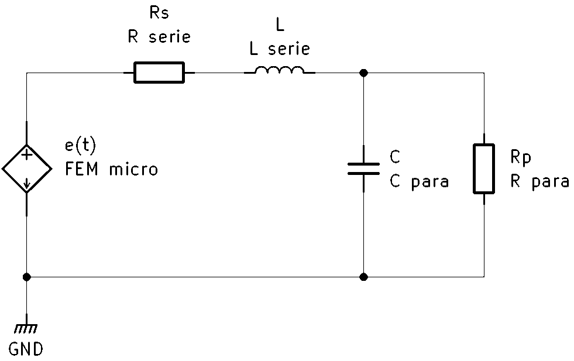
\includegraphics[width=0.8\textwidth]{../../../Attachment/Schema/01-Schema-eq-mic.png}
    \caption{Equivalent electrical circuit of an unloaded pickup}
\end{figure}

The pickup impedance can then be calculated as:
\begin{equation}
|Z(j\omega)| = \frac{1}{\sqrt{\left(\frac{1}{R_p} + \frac{R_s}{R_s^2 + (L\omega)^2}\right)^2 + \left(C\omega - \frac{L\omega}{R_s^2 + (L\omega)^2}\right)^2}}
\end{equation}

In actual use, the pickup is connected to an amplifier whose input resistance is modeled by a load $R_{amp}$. Studying this circuit makes it possible to establish the transfer function $H(p) = \frac{u(p)}{e(p)}$. We obtain the following expression:
\begin{equation}
H(p) = \frac{R_p R_{amp}}{R_p R_{amp} + R_s R_{amp} + R_s R_p} \frac{1}{1 + \frac{R_s R_p R_{amp} C + L R_{amp} + L R_p}{R_p R_{amp} + R_s R_{amp} + R_s R_p}p + \frac{R_p R_{amp} L C}{R_p R_{amp} + R_s R_{amp} + R_s R_p}p^2}
\end{equation}
This equation shows that, once loaded, the pickup behaves as a second-order low-pass filter.

\subsection{Experiment}
The objective of this first experimental phase is to characterize the physical parameters $R_s$, $L$, $C$, and $R_p$ introduced in the preceding theoretical model (1.1). These values, which depend on the winding geometry and design, are determined using a frequency-identification method.

\subsubsection{Experimental protocol}
The setup is based on a voltage-divider circuit. The pickup is placed in series with a precision resistor $R_{amp} = 100k\Omega$. By applying a sinusoidal voltage $U$ with constant amplitude and variable frequency, we measure the voltage $V$ across the pickup. The magnitude of the pickup impedance $|Z|$ is then obtained from the following relation:
$$|Z| = \frac{V R_{amp}}{U-V}$$

\begin{figure}[H]
    \centering
    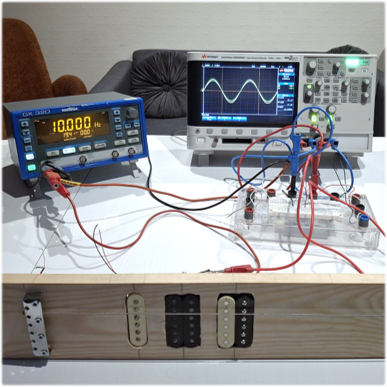
\includegraphics[width=0.8\textwidth]{../../../Test/Main/01-Elec.png}
    \caption{Photograph of the experimental setup}
\end{figure}

\subsubsection{Data processing and optimization}
The series resistance $R_s$ is first measured in direct current using a multimeter. The other parameters $L$, $C$, and $R_p$ are obtained by numerically fitting the theoretical model to the experimental points (Fig. 3). For this purpose, we use the least-squares algorithm, which minimizes the squared difference between prediction and measurement (Fig. 4).

\subsubsection{Results}
The results obtained for the two types of pickups studied are summarized in the table below:

\begin{center}
\begin{tabular}{lcccc}
\toprule
\textbf{Pickup type} & $\boldsymbol{R_s}$ & \textbf{L} & \textbf{C} & $\boldsymbol{R_p}$ \\
\midrule
SingleCoil & 5,26 k$\Omega$ & 2,37 H & 0,37 nF & 492,3 k$\Omega$ \\
Parallel Humbucker & 4,52 k$\Omega$ & 1,72 H & 0,05 nF & 343,0 k$\Omega$ \\
Series Humbucker & 15,1 k$\Omega$ & 4,60 H & 0,11 nF & 1,05 M$\Omega$ \\
\bottomrule
\end{tabular}
\end{center}

Examination of the impedance curves (Fig. 3) confirms the resonant nature of the three devices studied: the SingleCoil, the Humbucker in parallel configuration, and the Humbucker in series configuration. The experimental results reveal that the resonance frequency of the series Humbucker is significantly higher than that of the SingleCoil, in agreement with its low parasitic capacitance (0.11 nF), identified by the least-squares algorithm. In contrast, the parallel Humbucker, characterized by a parasitic capacitance of 0.05 nF and an inductance of 1.72 H, exhibits resonance at an intermediate frequency, distinct from the other two configurations.

Detailed analysis of the experimental readings reveals a pronounced asymmetry in the frequency response of the parallel Humbucker, in contrast with the symmetry of the resonance peak of the SingleCoil and series Humbucker.

\begin{figure}[H]
    \centering
    \begin{minipage}{0.48\textwidth}
        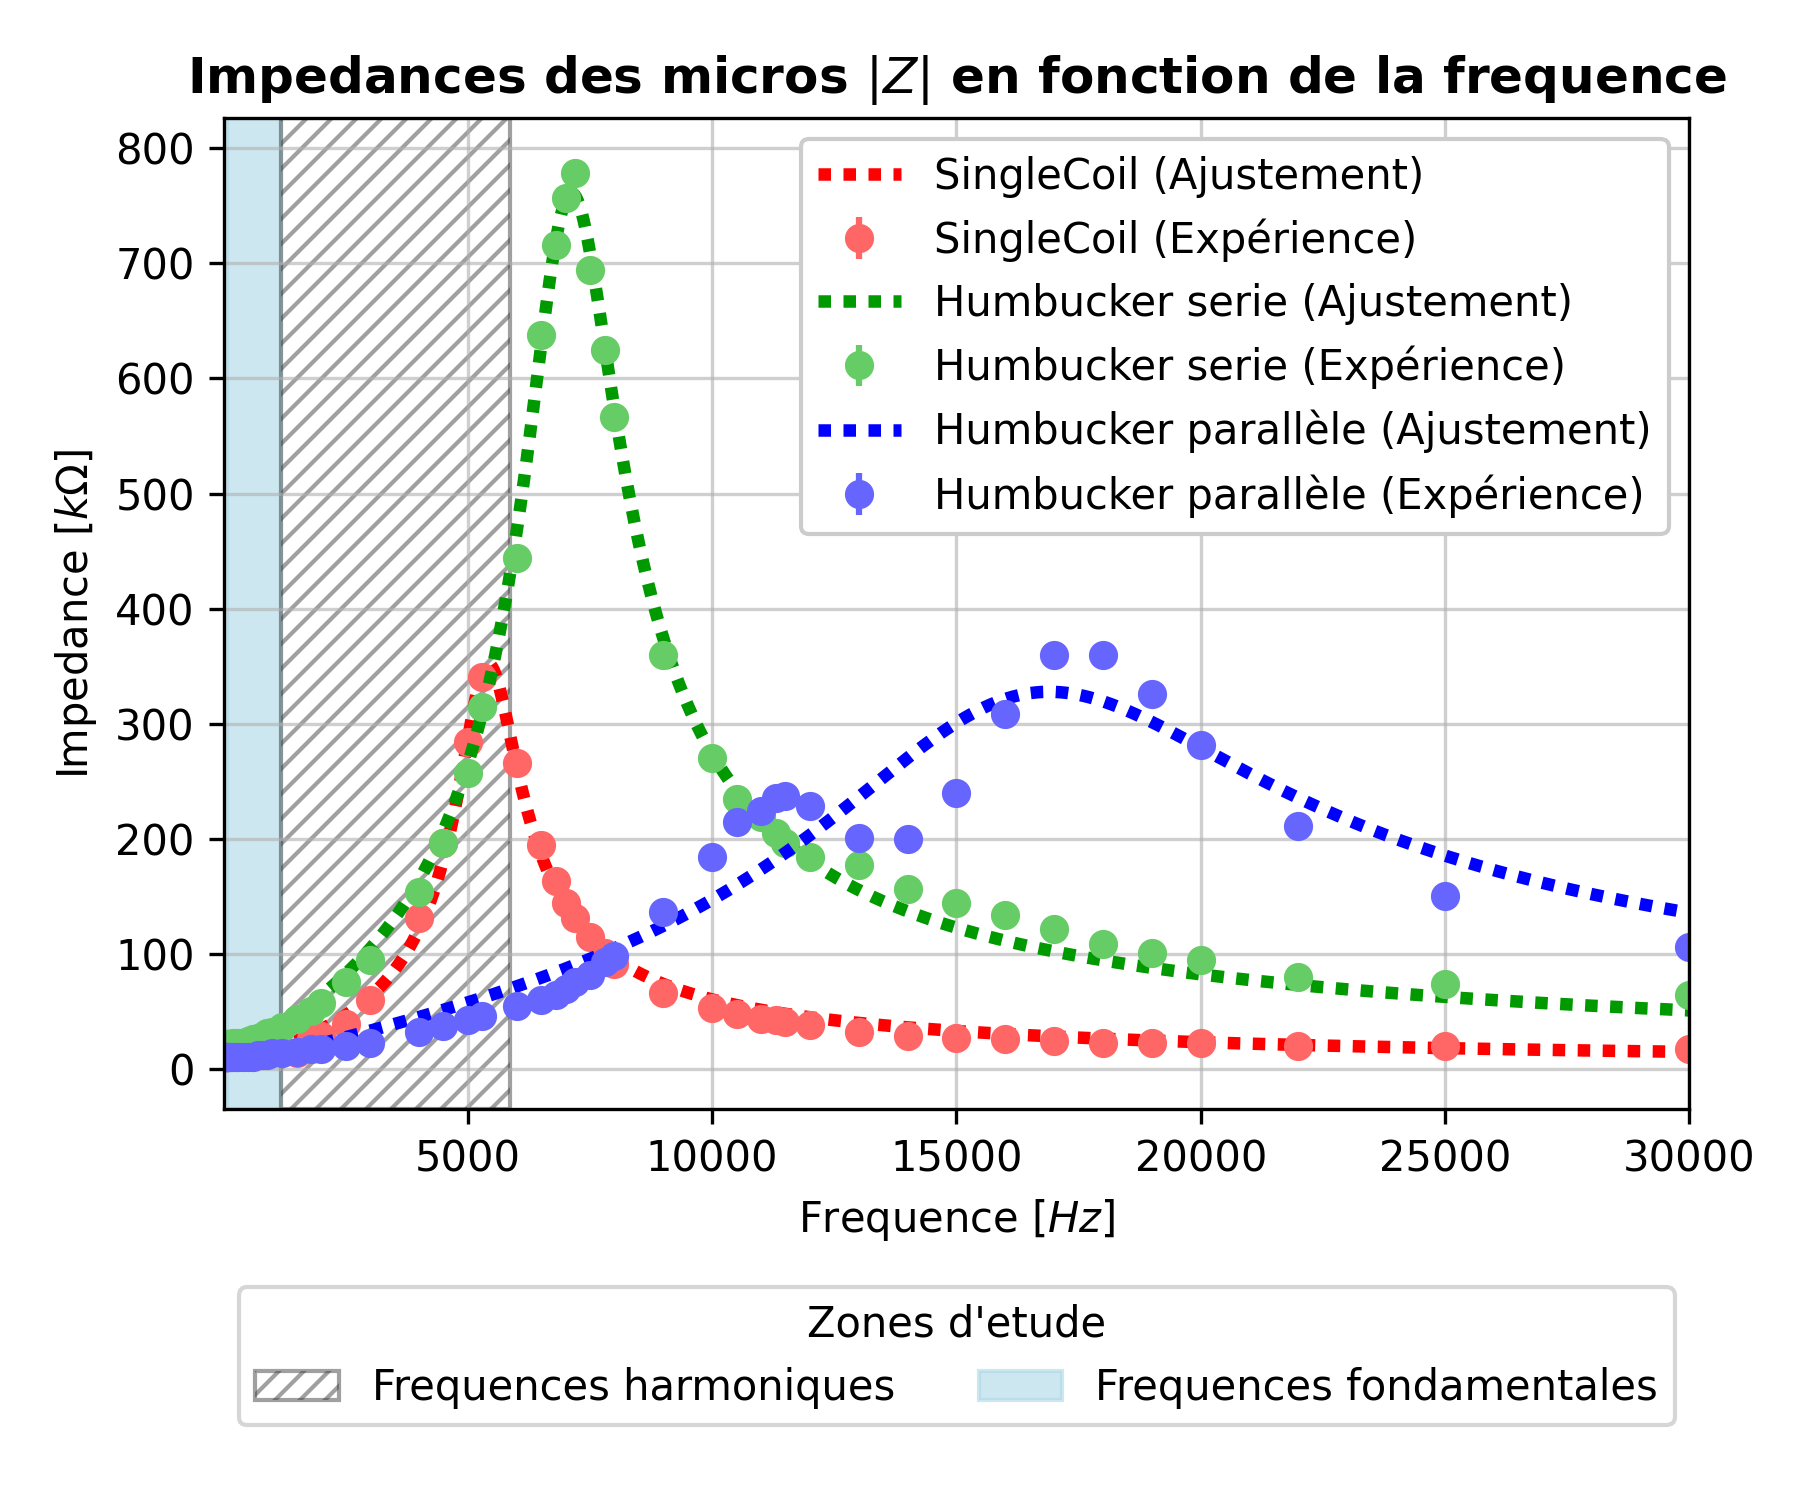
\includegraphics[width=\linewidth]{../../../Python/Exports/01-Reponse_electrique_frequetielle/Impedance.png}
        \caption{Experimental impedance readings}
    \end{minipage}\hfill
    \begin{minipage}{0.48\textwidth}
        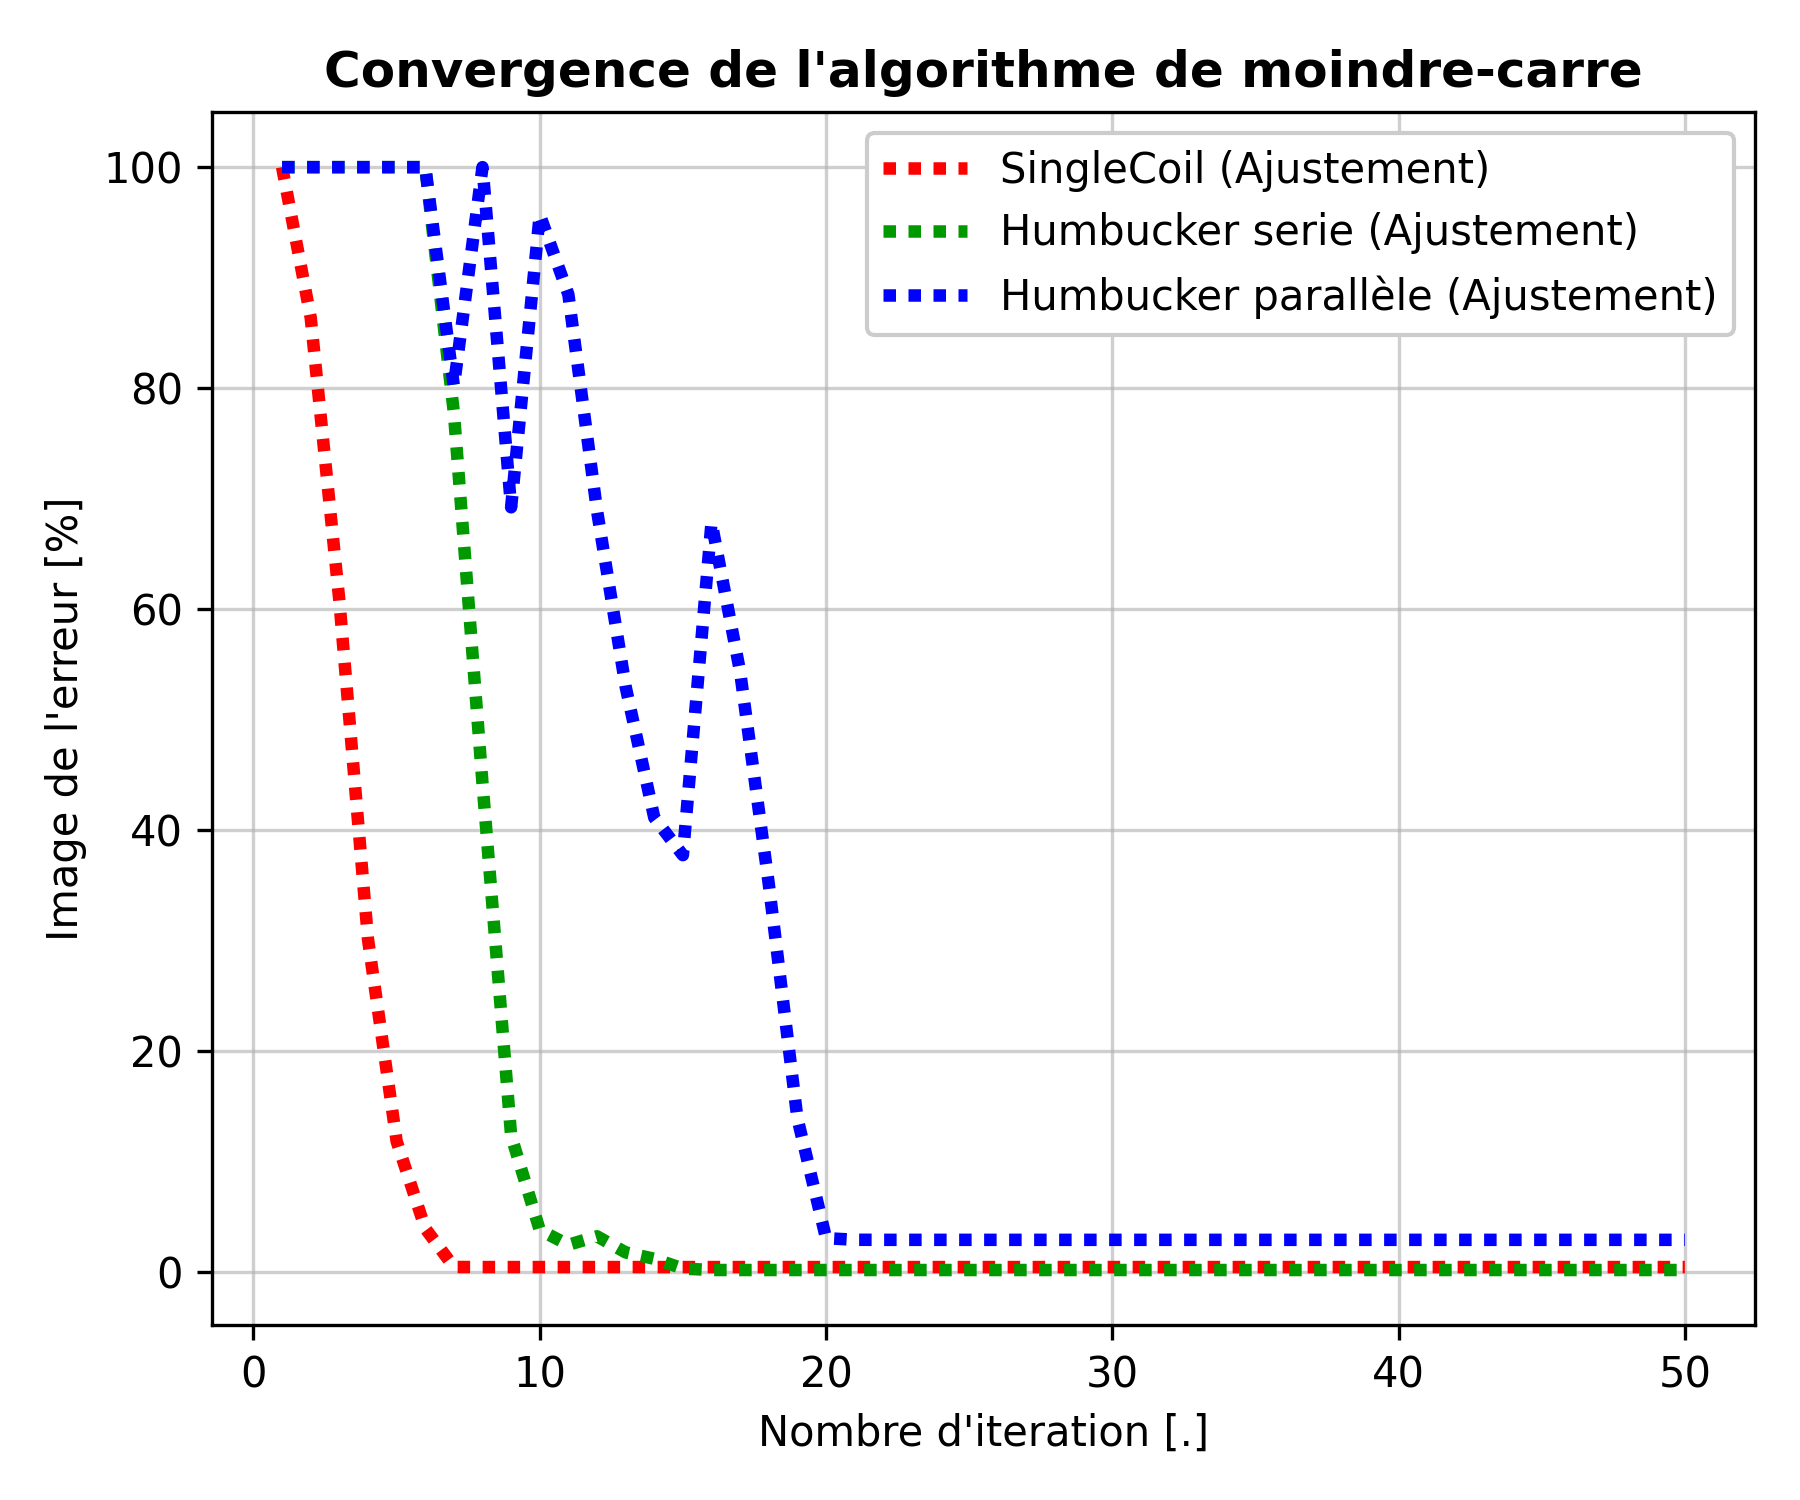
\includegraphics[width=\linewidth]{../../../Python/Exports/01-Reponse_electrique_frequetielle/Convergence.png}
        \caption{Convergence of the least-squares algorithm}
    \end{minipage}
\end{figure}

This singularity suggests that the standard second-order model, although adequate for describing the SingleCoil and series Humbucker, is insufficient for the parallel Humbucker. The shape of its impedance curve indicates behavior compatible with a fourth-order system, characteristic of an arrangement in which the two coils are not identical. This configuration profoundly modifies the transducer's frequency response, shifting the resonance towards high frequencies and introducing additional complexity into the signal's internal filtering.

Identifying the physical parameters now makes it possible to simulate the exact frequency behavior of each pickup when loaded by an amplifier $R_{amp} = 1M\Omega$. Figure 5 presents the Bode diagram obtained by numerical simulation.

\begin{figure}[H]
    \centering
    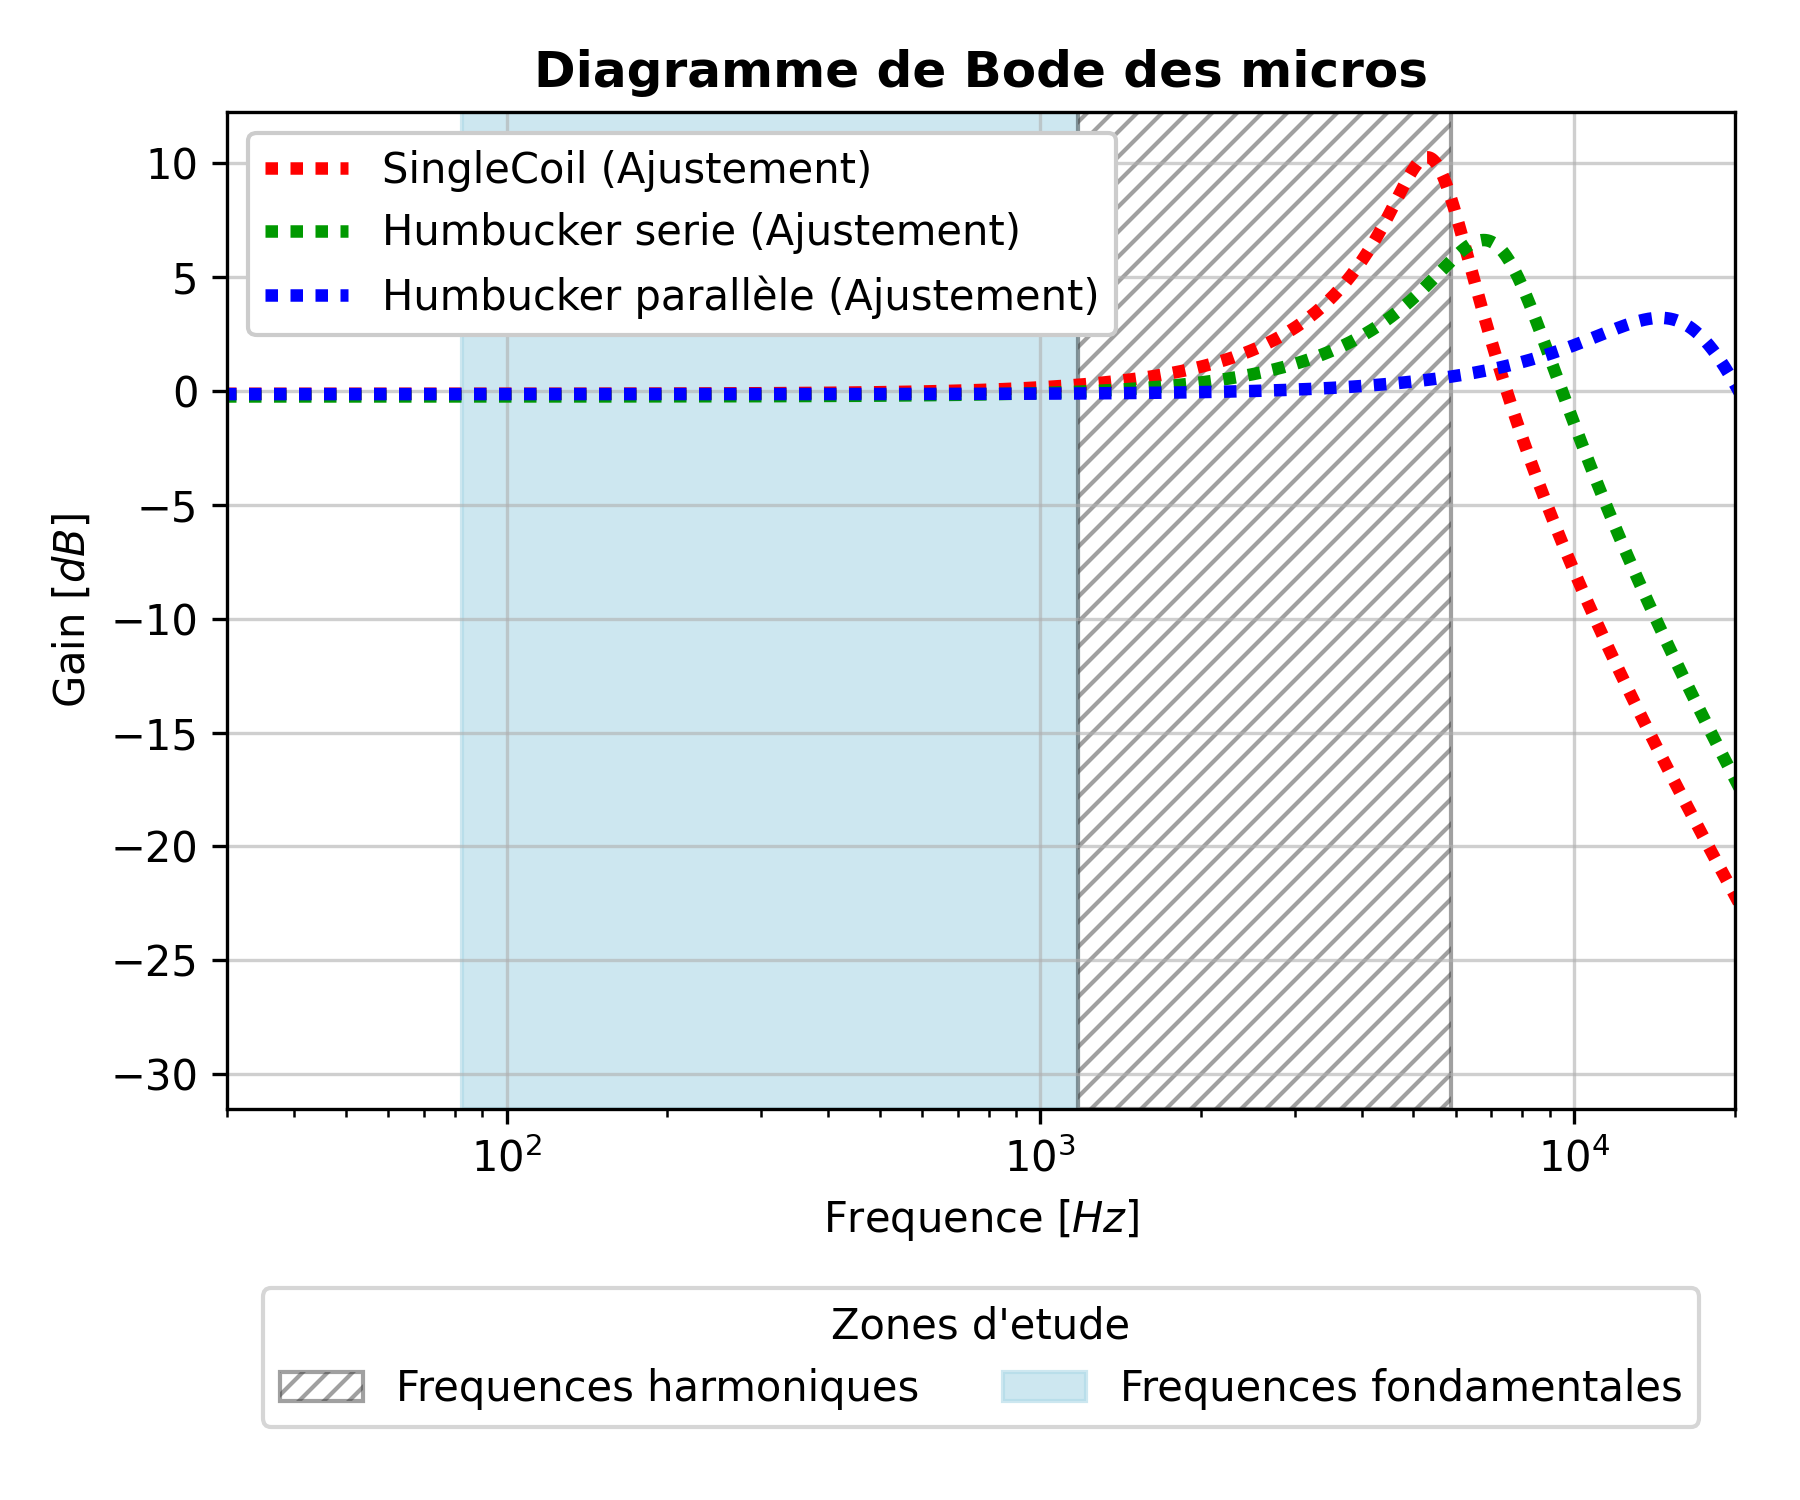
\includegraphics[width=0.8\textwidth]{../../../Python/Exports/01-Reponse_electrique_frequetielle/01-Gain.png}
    \caption{Bode diagram of the pickups}
\end{figure}

\subsection{Conclusion}
The SingleCoil pickup is distinguished by a pronounced resonance peak and a high quality factor, promoting the selective transmission of harmonics in the upper part of the audible spectrum. This characteristic gives this winding type its historically appreciated ``bright'' and ``sharp'' tone, in which the resonance boost enriches the string's original timbre.

Conversely, the parallel Humbucker has a frequency response without harmonic coloration in the audible midrange and treble. The resonance, shifted towards very high frequencies because of its low parasitic capacitance (0.05 nF), produces a more linear reproduction of the signal, but at the expense of treble harmonic enhancement. This configuration creates a sound perceived as ``darker'' and less rich in high frequencies, limited by the bandwidth of the amplification system.

The series Humbucker combines elements of the two preceding behaviors. With an intermediate parasitic capacitance (0.11 nF) and a higher inductance (4.60 H), it retains a more pronounced resonance than the parallel arrangement while attenuating treble harmonics relative to the SingleCoil. This configuration therefore offers a compromise between the brightness of the SingleCoil and the linearity of the parallel Humbucker, with a more balanced frequency response.

These fundamental differences between winding configurations illustrate how electrical architecture directly influences the guitar's timbre. The choice between SingleCoil, parallel Humbucker, and series Humbucker will therefore depend on the musician's sound preferences, as well as on the technical constraints associated with the operating environment.

\newpage
% --- SECTION II ---
\section{Induction and spatial filtering}

\subsection{Theory}
\subsubsection{String vibration}
The study of electromagnetic transduction is based on a precise characterization of the vibration of the ferromagnetic string and its interaction with the pickup's static magnetic field. In accordance with the work of B. d'Andréa-Novel, B. Fabre, and P. Jouvelot [6], the vertical displacement of the string $z(x,t)$ at a point $x$ and at time $t$ can be modeled as a superposition of standing waves. The general expression for the motion is therefore:
\begin{equation}
z(x,t) = z_0 + \sum_{n} B_n \sin(k_n x) \cos(2\pi n F t)
\end{equation}
In this equation, $z_0$ represents the equilibrium position of the string relative to the pickup, while $B_n$ denotes the amplitude of the $n^{\text{th}}$ harmonic. This amplitude depends closely on the initial plucking conditions, in particular the initial amplitude $A_0$ and the excitation position $x_0$ along the vibrating length $L$. The wave number $k_n$ is expressed as $k_n = n\pi/L$. The relation governing these amplitudes is:
\begin{equation}
B_n = \frac{A_0 L^{5/2} \sqrt{2}}{\pi^2 x_0 (L - x_0)} \frac{\sin\left(\frac{n\pi x_0}{L}\right)}{n^2}
\end{equation}

\subsubsection{Induction}
Consider a portion of the string with volume $V$ and magnetic susceptibility $\chi$, placed in the magnetic field $\vec{B_m}$ of the pickup's permanent magnet. This portion of string therefore acquires a magnetic moment $\vec{m}$ such that:
\begin{equation}
\vec{m} = \frac{\chi V \vec{B_m}}{\mu_0}
\end{equation}
In the dipole approximation, and considering the magnetic moment to be vertically aligned, the field $\vec{B_c}$ created by this magnetic moment at a distance $z$ is given by:
\begin{equation}
\vec{B_c}(z) = \frac{\mu_0}{4\pi} \frac{2\vec{m}}{z^3} = \frac{\chi V \vec{B_m}(z)}{2\pi z^3}
\end{equation}
Thus, the magnetic flux $\Phi$ passing through the $N$ turns with cross-sectional area $S$ is expressed as:
\begin{equation}
\Phi(z,t) = N \oint \vec{B_c}(z,t) \cdot \vec{dS} = \frac{N S \chi V}{2\pi} \frac{B_m(z)}{z(t)^3}
\end{equation}
Applying Faraday's law of induction finally makes it possible to determine the electromotive force $e(x,t)$ induced in the pickup. Decomposing the time derivative of the flux using the chain rule, namely $e(t) = -\frac{\partial\Phi}{\partial t} = -\frac{\partial\Phi}{\partial z}\frac{\partial z}{\partial t}$, we obtain the final expression for the electrical signal:
\begin{equation}
e(x,t) = \frac{N S \chi V}{2\pi} \left( \frac{3B_m(z(t))}{z^4} - \frac{1}{z^3} \frac{\partial B_m}{\partial z}(t) \right) \sum_{n} B_n 2\pi n F \sin(k_n x) \sin(2\pi n F t)
\end{equation}
Thus:
\begin{equation}
e(x,t) = \frac{N S \chi V}{2\pi} \left( \frac{3B_m(z(t))}{z^4} - \frac{1}{z^3} \frac{\partial B_m}{\partial z}(t) \right) \sum_{n} B_n A_n \sin(2\pi n F t)
\end{equation}
This formulation demonstrates that the induced voltage is directly proportional to the string's vibration velocity and depends on the pickup's spatial position along the string. This spatial dependence is the origin of the comb-filtering phenomenon, which will be analyzed in the following section to compare SingleCoil and Humbucker pickups.

\subsection{Experiment}
Validation of the induction model is based on a series of time-domain and frequency-domain measurements performed using an instrumented guitar model (Fig. 6). The manually excited string vibrates at a fundamental frequency of 80 Hz. Observation of the time-domain signals (Fig. 7) shows an overall correlation between theory and experiment, although notable morphological differences appear, particularly at certain specific frequencies.

\begin{figure}[H]
    \centering
    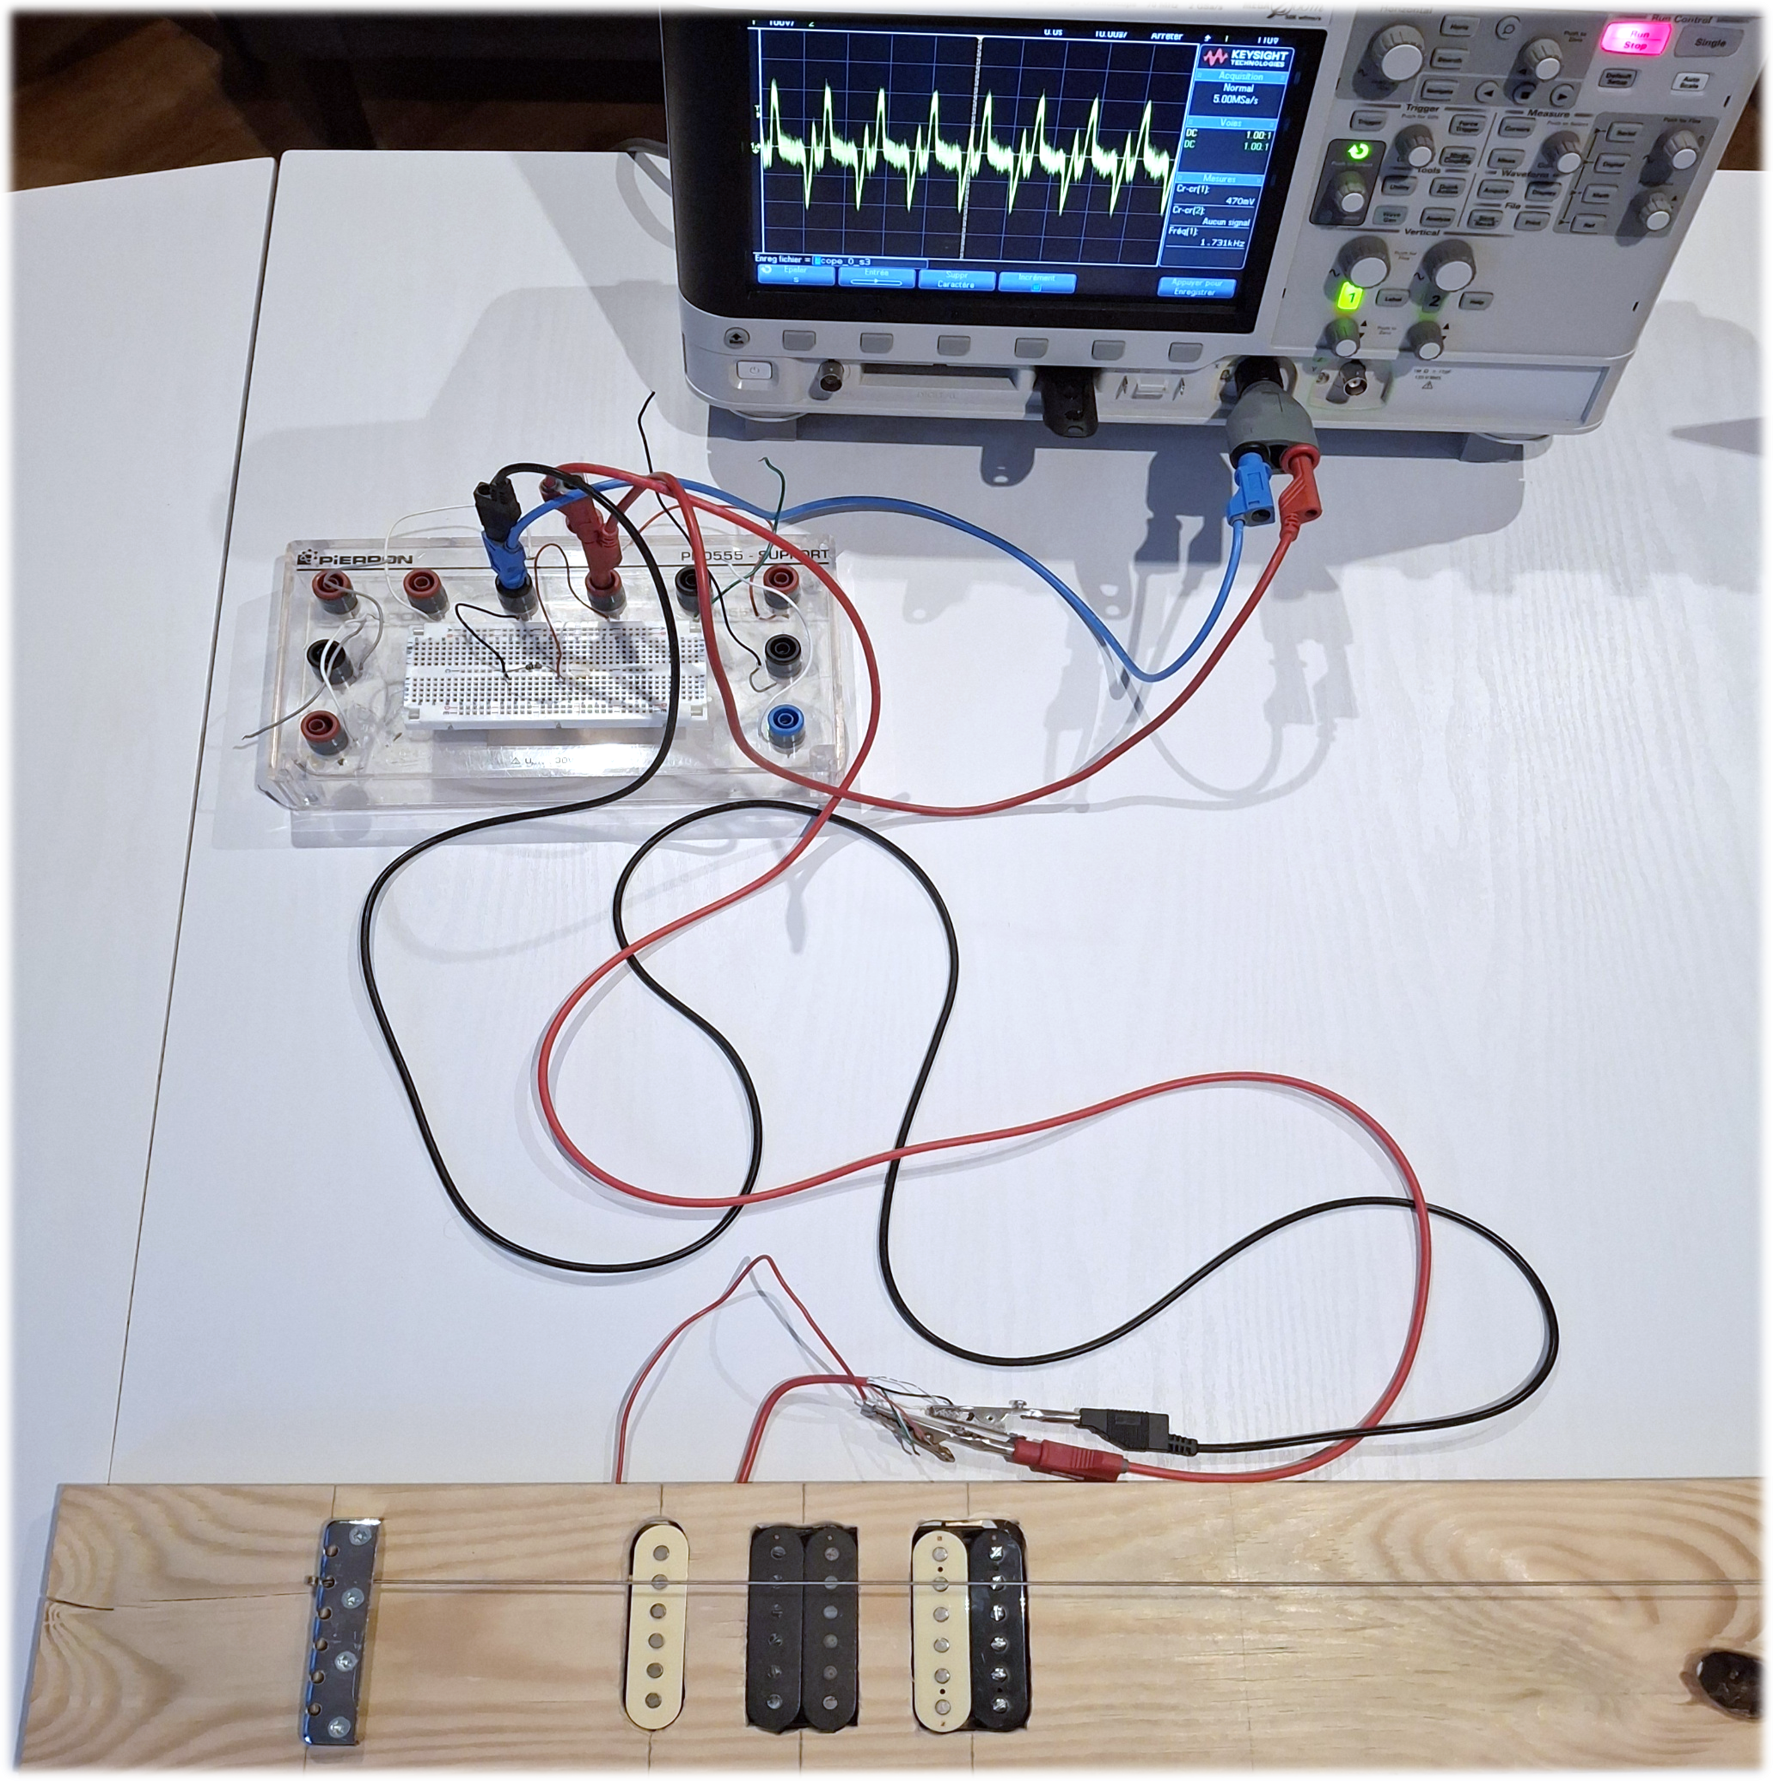
\includegraphics[width=0.5\textwidth]{../../../Test/Main/02-Meca.png}
    \caption{Photograph of the experimental setup}
\end{figure}

\begin{figure}[H]
    \centering
    \begin{minipage}{0.48\textwidth}
        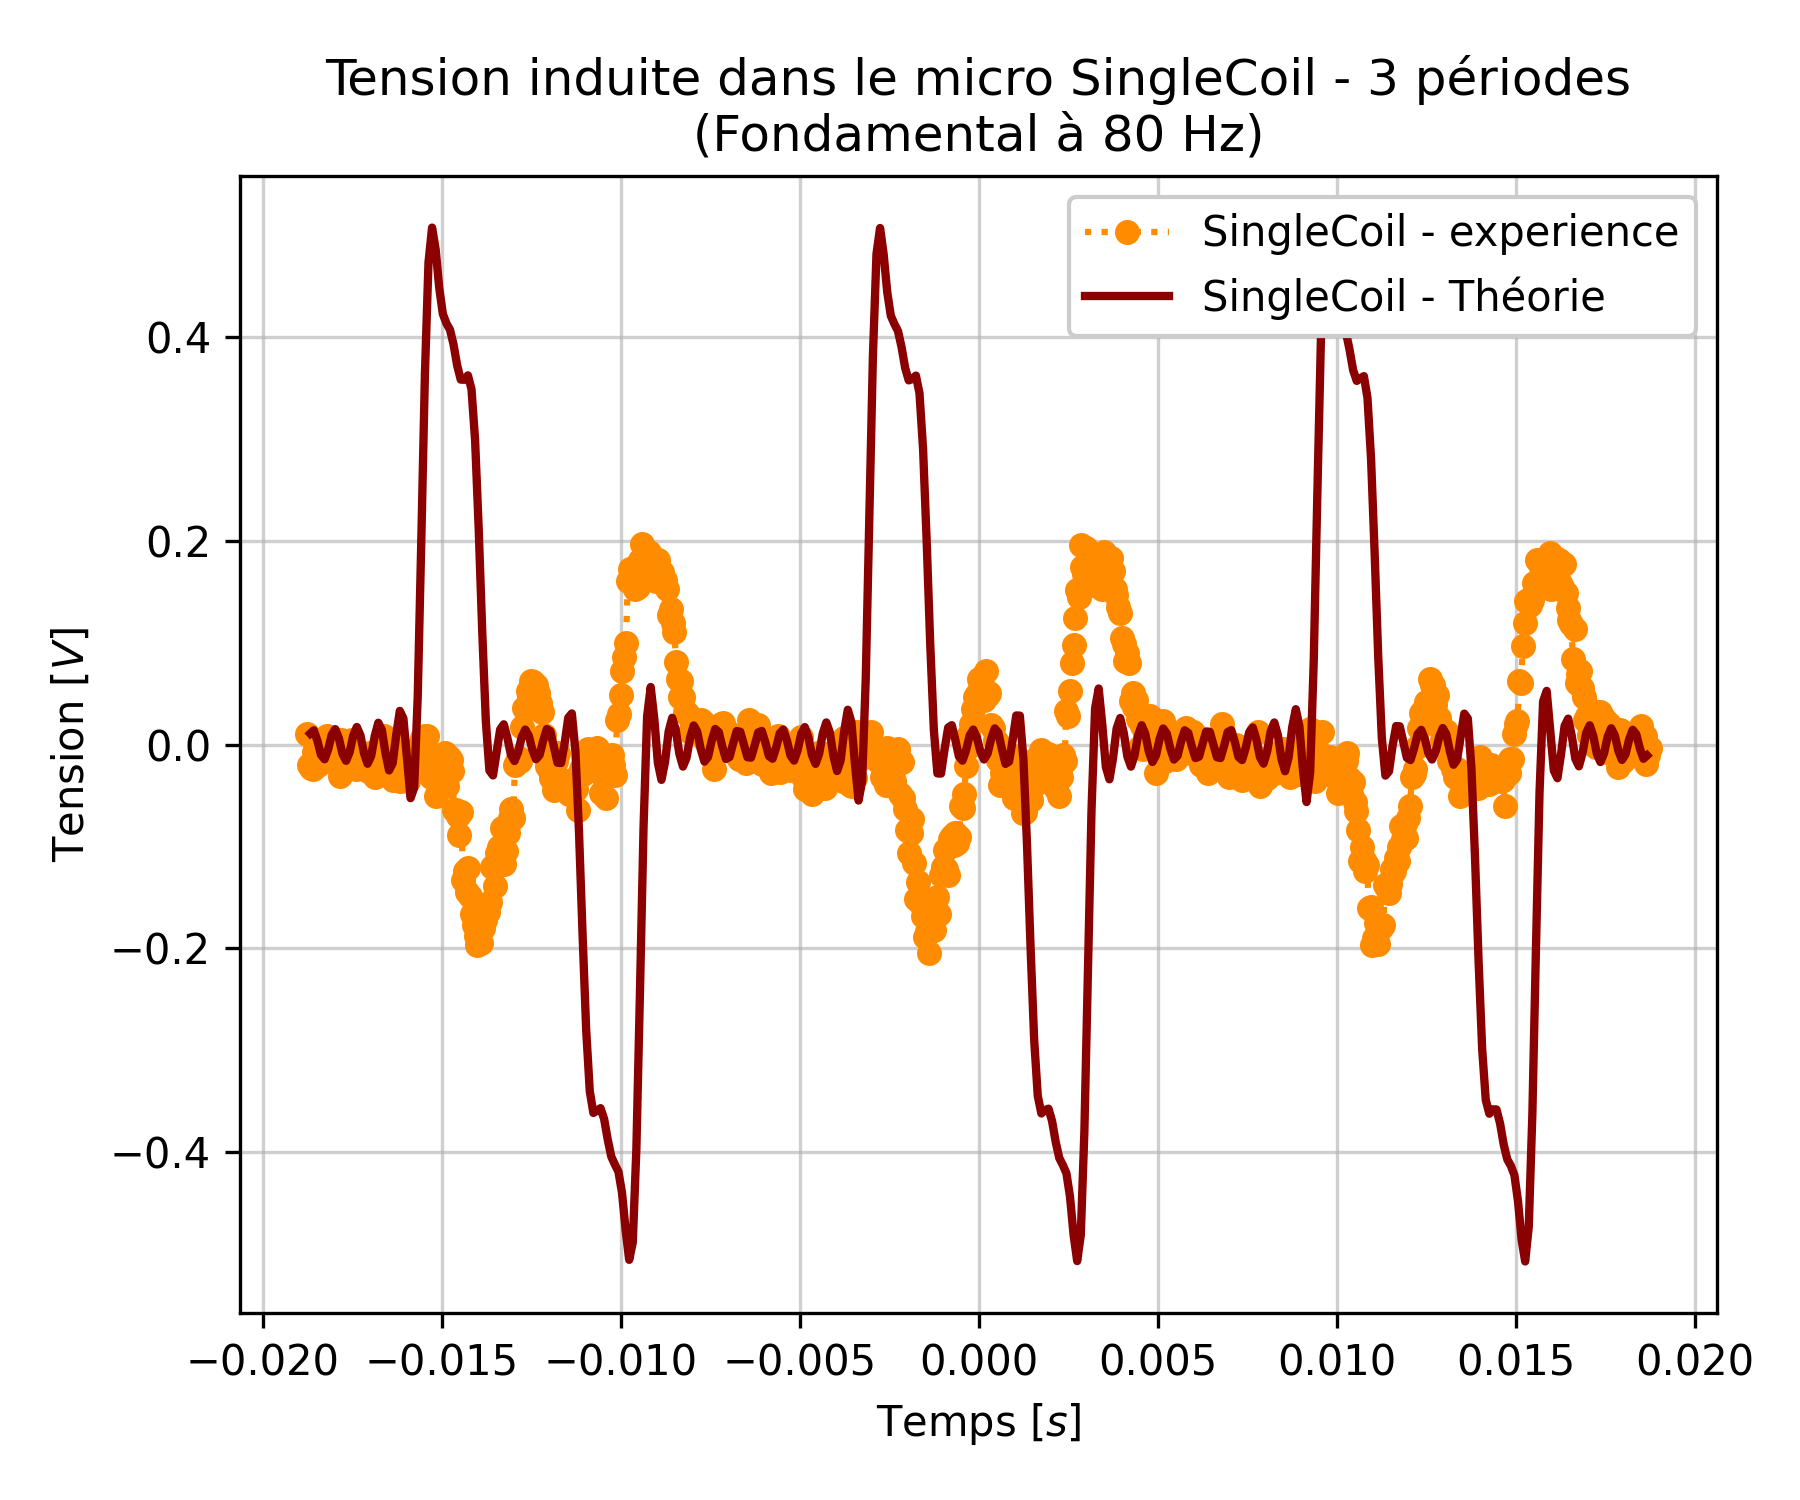
\includegraphics[width=\linewidth]{../../../Python/Exports/02-Reponse_mecanique/temporel/Singlecoil.png}
        \caption{Time response of the pickup to string excitation}
    \end{minipage}\hfill
    \begin{minipage}{0.48\textwidth}
        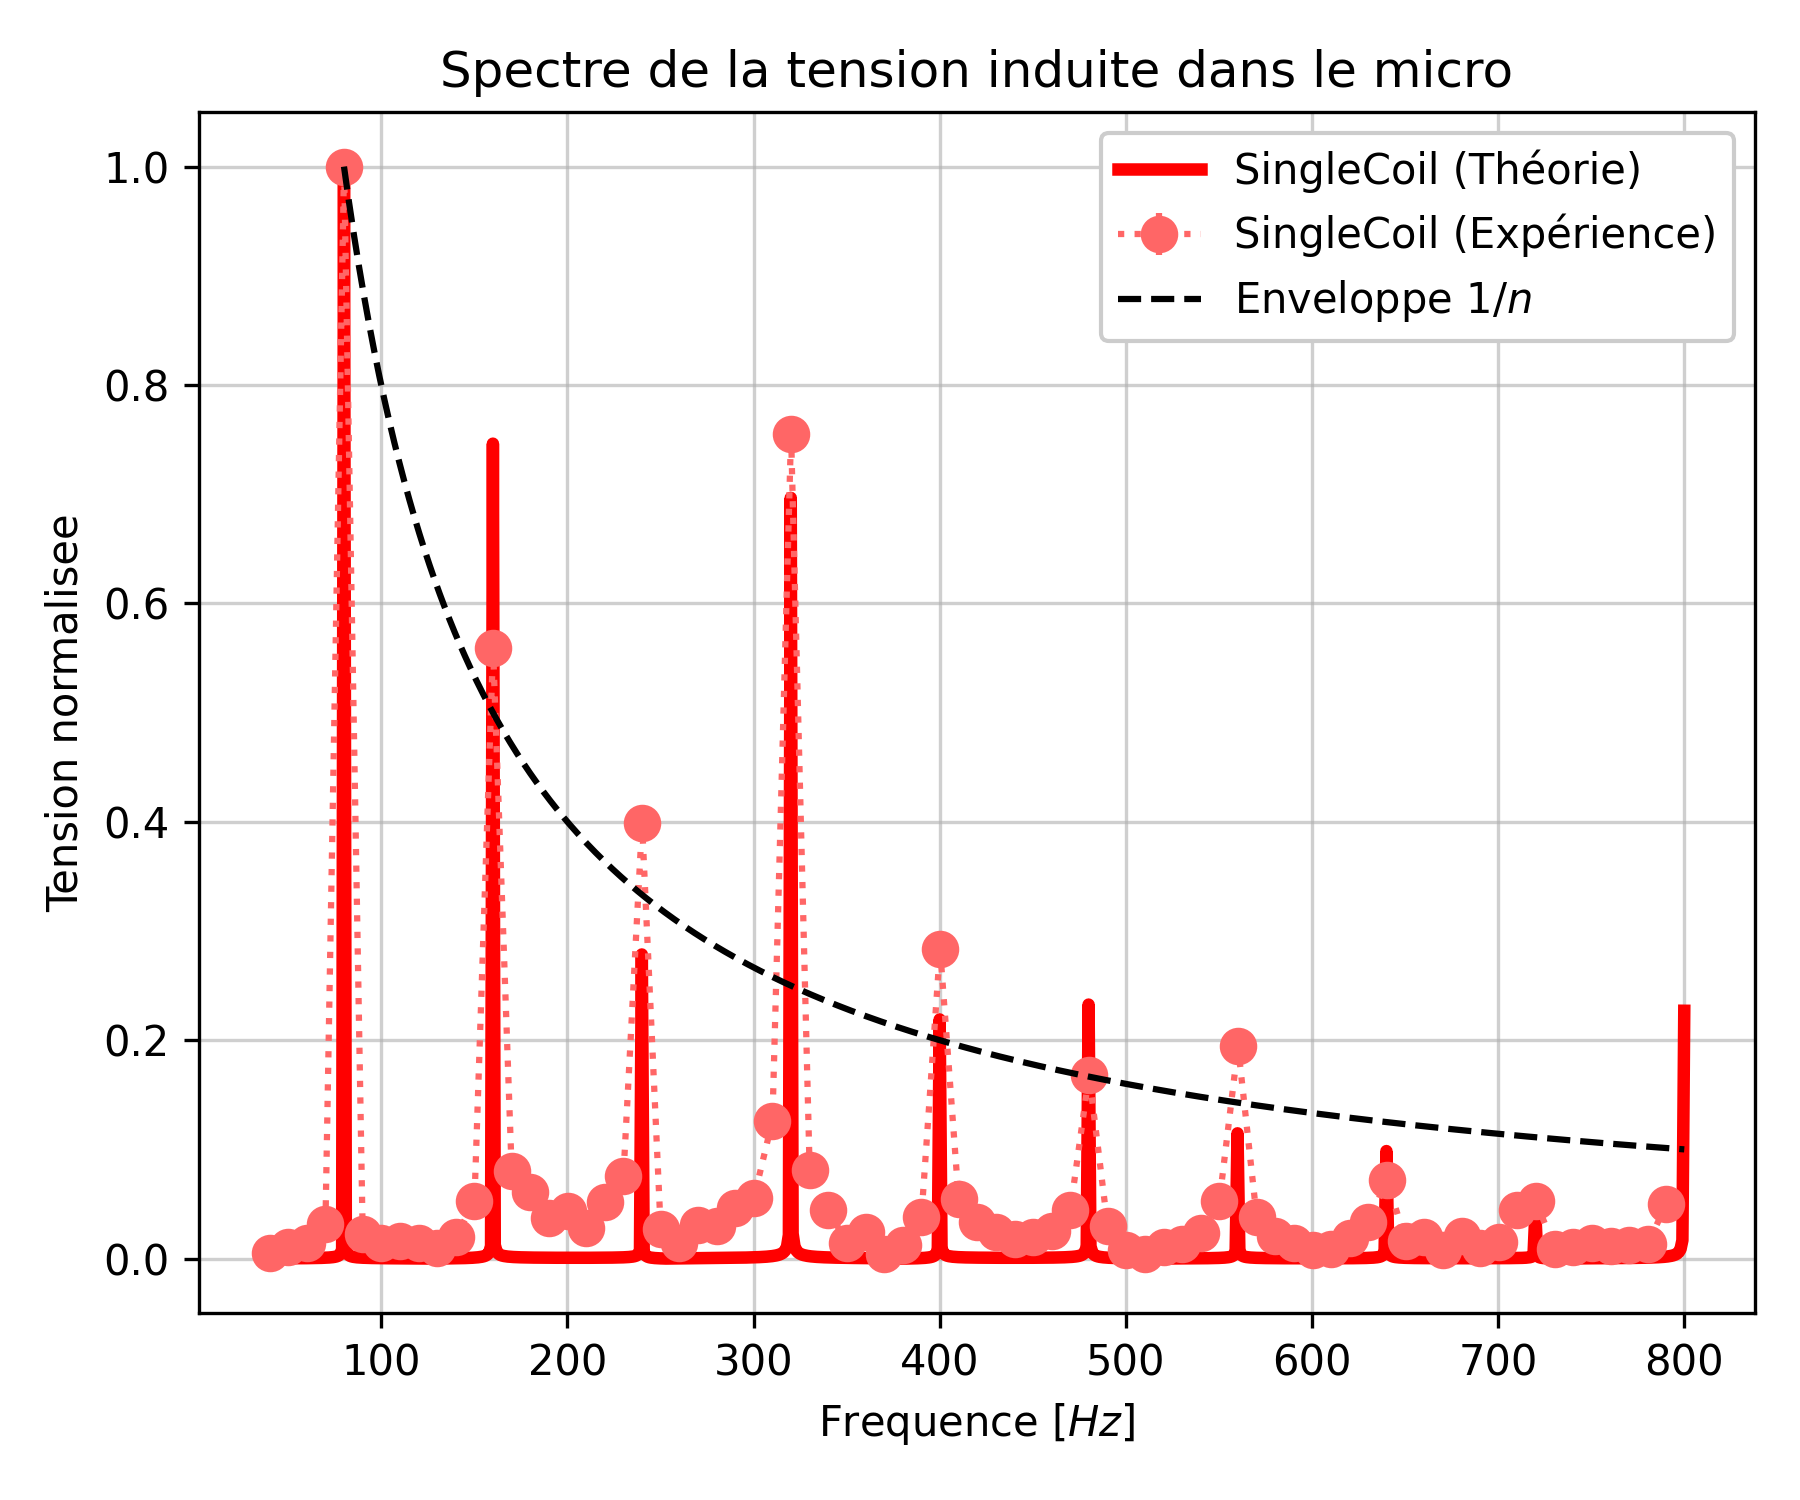
\includegraphics[width=\linewidth]{../../../Python/Exports/02-Reponse_mecanique/FFT/SC/Singlecoil.png}
        \caption{Spectral response of the pickup to string excitation}
    \end{minipage}
\end{figure}

Spectral analysis of the signals (Fig. 8) confirms the presence of higher-order harmonics, in accordance with the predictions of the Fourier series expansion. However, the experimental amplitudes differ from the theoretical values obtained from the dipole model, particularly at certain frequencies. These differences can be explained by several phenomena.

Manual excitation of the string introduces an initial plucking condition that is not ideally triangular. Unlike the theoretical model, which assumes that harmonic amplitudes decrease as $1/n$, this excitation produces a richer and more complex harmonic spectrum, changing the energy distribution between the fundamental frequencies and their harmonics.

The theoretical model treats the pickup as a point sensor, thereby neglecting the integration of magnetic flux over the finite surface of the pole pieces. In reality, the non-negligible dimensions of the coils introduce spatial low-pass filtering: harmonics whose wavelength is comparable to the size of the pole piece undergo additional attenuation, altering the measured frequency response.

The model assumes a constant magnetic-field gradient $\frac{\partial B_m}{\partial z}$. However, for large vibration amplitudes, the string enters regions of magnetic saturation near the magnets, where the field is no longer linear. This phenomenon causes distortion of the time-domain signal, appearing as sharper and more aggressive voltage peaks on the oscilloscope, in contrast with the smoothed curves from the simulations.

\subsection{Conclusion}
The comparative study of SingleCoil and Humbucker technologies highlights the decisive impact of winding geometry on the electric guitar's timbre. Thanks to its point-like capture of vibrations, the SingleCoil preserves the entire harmonic spectrum, giving the sound its characteristic brightness and richness in high frequencies.

By contrast, the Humbucker, through its dual structure, introduces spatial comb filtering related to the spacing $\Delta$ between its two coils. This physical phenomenon generates destructive interference for vibrational wavelengths whose antinodes are in phase opposition between the coils. Certain harmonics are therefore attenuated, acting as a passive equalizer that actively shapes the spectral content of the signal.

\begin{figure}[H]
    \centering
    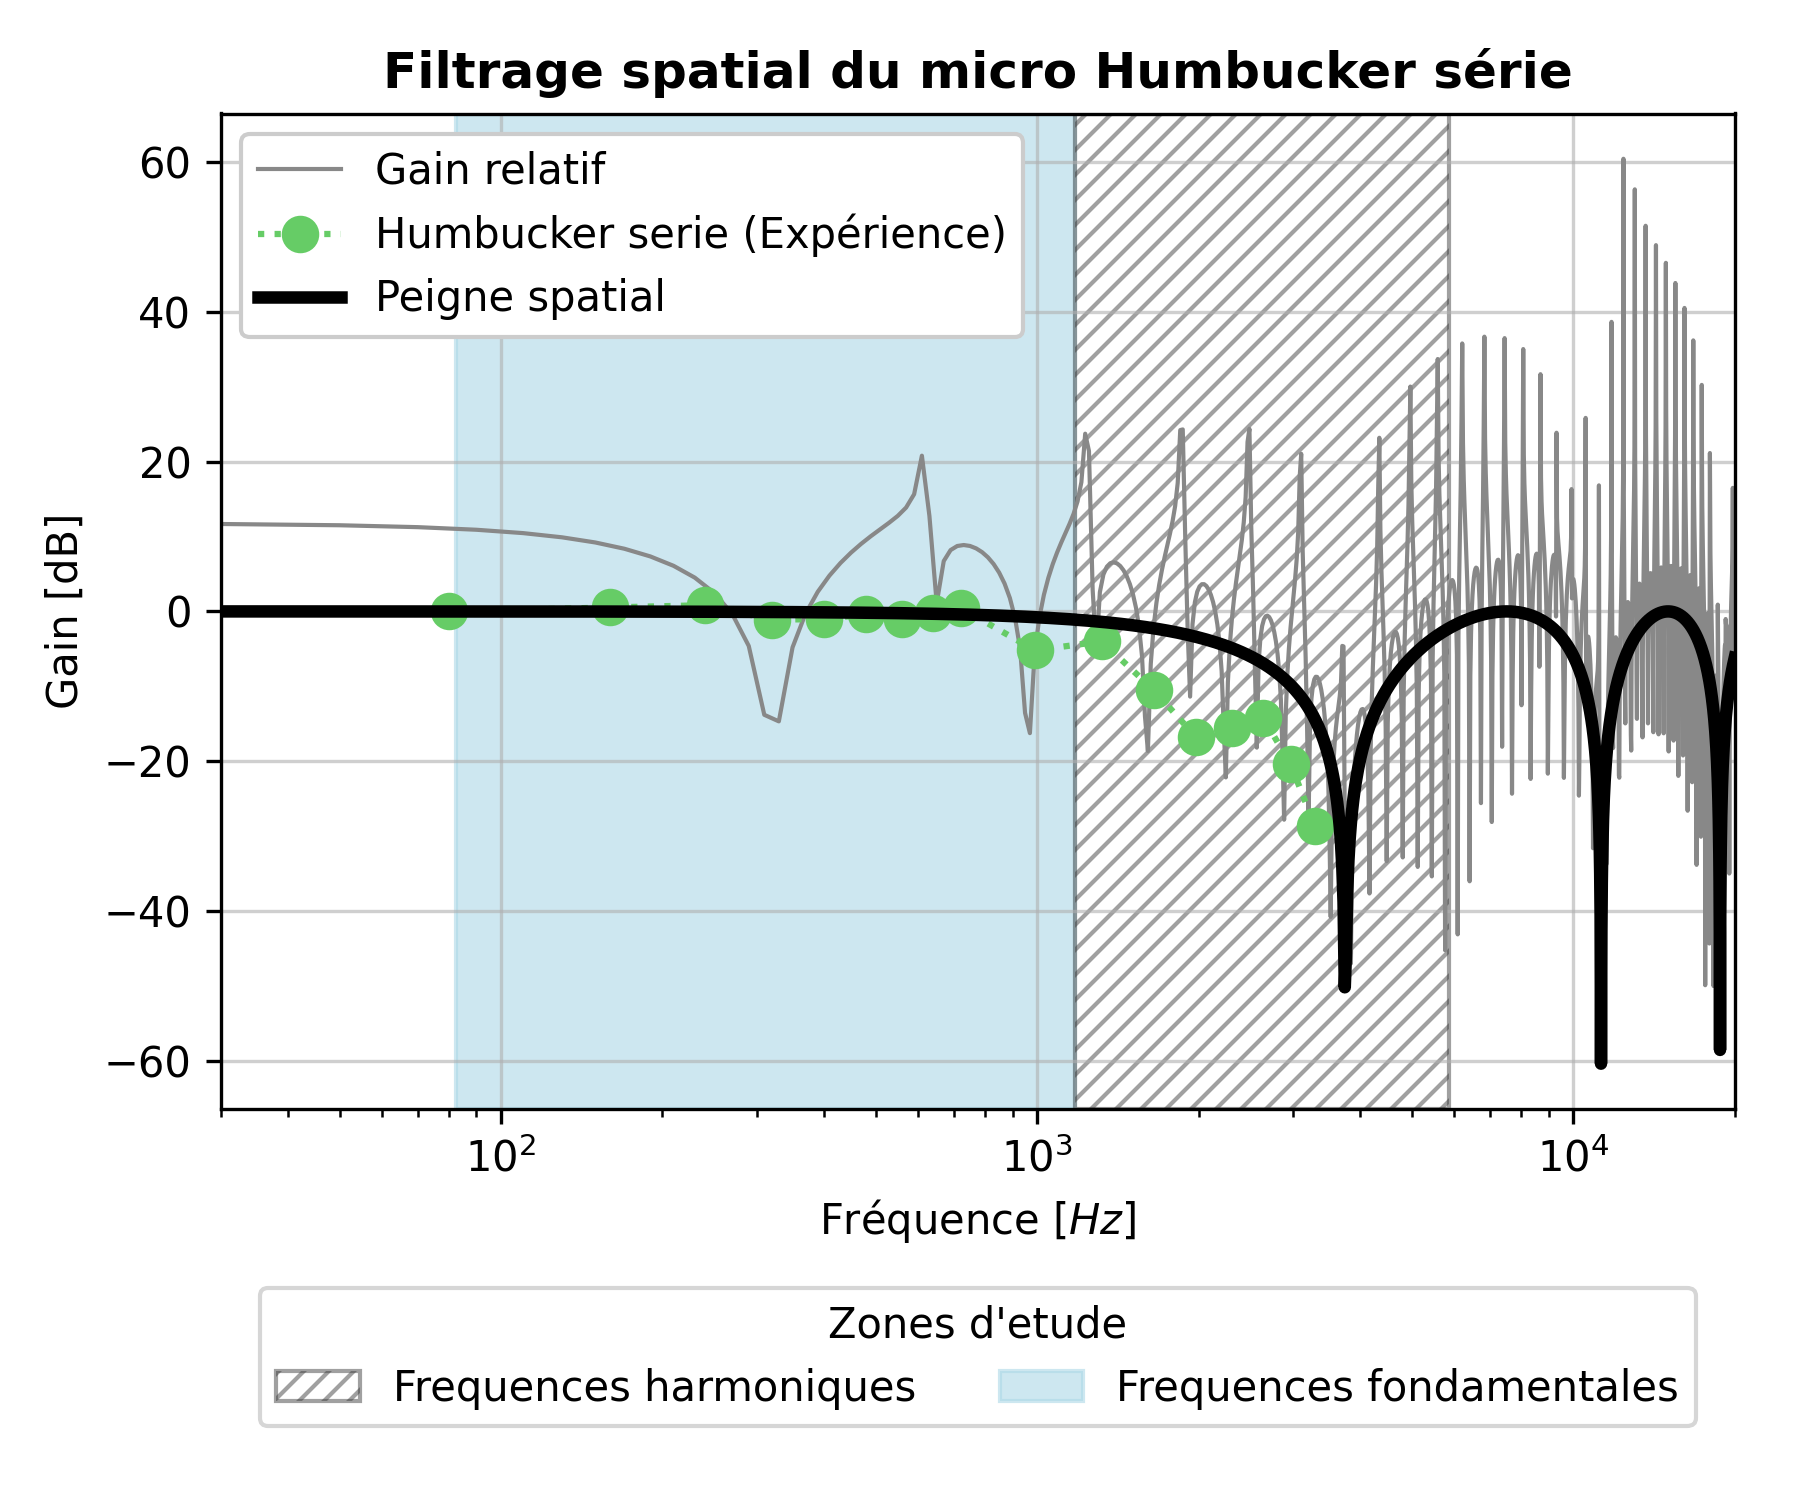
\includegraphics[width=0.8\textwidth]{../../../Python/Exports/02-Reponse_mecanique/Filtrage_spatial.png}
    \caption{Spatial comb filtering of the Humbucker pickup}
\end{figure}

This spatial filtering, combined with the electrical filtering studied in Part 1, scientifically explains the Humbucker's more ``dull'' and ``round'' tone. The dual coil is therefore not limited to simply reducing interference: it reshapes the instrument's acoustic identity by altering the very structure of the induced signal, illustrating the fundamental compromise between sound purity and harmonic richness.

\newpage
% --- SECTION III ---
\section{Hum reduction}

\subsection{Theory}
Studying an electromagnetic sensor's sensitivity to environmental noise requires modeling the interfering magnetic field as a non-uniform alternating field. In the pickup's reference frame, this field, mainly induced by 50 Hz mains radiation, is described by its local amplitude $B_0$, its frequency $F_B$, and its spatial gradient $\alpha$ along the guitar's longitudinal axis. Considering only the component normal to the turns, the simplified expression of the interfering field is:
\begin{equation}
B(x',t) = B_0(1 + \alpha x') \cos(2\pi F_B t)
\end{equation}
where $x'$ represents the spatial position relative to the pickup's center of gravity.

\subsubsection{SingleCoil pickup}
In a SingleCoil pickup configuration, the winding is centered at $x' = 0$. Applying Lenz-Faraday's law of induction makes it possible to express the induced electromotive force (EMF) $e_S(t)$ as a function of the number of turns $N_S$ and the active area $S$. The resulting EMF is directly proportional to the amplitude of the incident field:
\begin{equation}
e_S(t) = N_S S B_0 2\pi F_B \sin(2\pi F_B t)
\end{equation}
This result demonstrates the absence of intrinsic filtering: the pickup captures the entire ambient electromagnetic noise, generating the characteristic hum observed experimentally (Fig. 11).

\subsubsection{Humbucker pickup}
The Humbucker pickup is based on the principle of phase-opposed wiring of two identical coils separated by a distance $\Delta$. The total EMF $e_H(t)$ is then the difference between the voltages induced in each coil, located respectively at $x'_1 = \frac{\Delta}{2}$ and $x'_2 = -\frac{\Delta}{2}$. By algebraically summing the contributions, the constant terms in $B_0$ cancel each other through phase opposition. Only a residual term dependent on the spatial gradient of the field remains:
\begin{equation}
e_{HS}(t) = N_{HS} S B_0 2\pi F_B \alpha \Delta \sin(2\pi F_B t)
\end{equation}
\begin{equation}
e_{HP}(t) = \frac{1}{2} N_{HP} S B_0 2\pi F_B \alpha \Delta \sin(2\pi F_B t)
\end{equation}
This demonstration highlights the Humbucker's effectiveness: in a perfectly uniform field ($\alpha = 0$), the interfering noise is theoretically zero. In practice, the interfering field always has slight inhomogeneity, but the term remains far below unity, ensuring massive noise attenuation compared with the SingleCoil pickup. This common-mode rejection property is the major technical advantage of this winding type in electromagnetically polluted environments.

\subsection{Experiment}
\subsubsection{Setup and protocol}
To validate the theoretical model of common-mode rejection, an experimental setup based on a Helmholtz coil system was implemented (Figure 10). This arrangement generates, at the center of the device, an alternating magnetic field whose amplitude and frequency are precisely controlled by a function generator. By placing the pickups at the center of these coils, we ensure an environment in which the magnetic field is nearly uniform, tending to minimize the spatial gradient $\alpha$ in accordance with the theoretical assumptions established above. To simulate real operating conditions, the pickups are connected to a load resistance $R_{amp}$ of 1 M$\Omega$, modeling the input impedance of a standard amplifier, and the induced voltage $u(t)$ is measured across this resistance using an oscilloscope.

\begin{figure}[H]
    \centering
    \includegraphics[width=0.8\textwidth]{PATH}
    \caption{Photograph of the experimental setup}
\end{figure}

\subsubsection{Time-domain results}
The pickups' sensitivity to external fields is characterized by a proportionality coefficient $k$ such that:
\begin{equation}
|e| = k |B|
\end{equation}
Measurements performed under an interfering field of variable amplitude at a frequency of 50 Hz reveal a major difference between the two technologies (Fig. 11).

\begin{figure}[H]
    \centering
    \begin{minipage}{0.48\textwidth}
        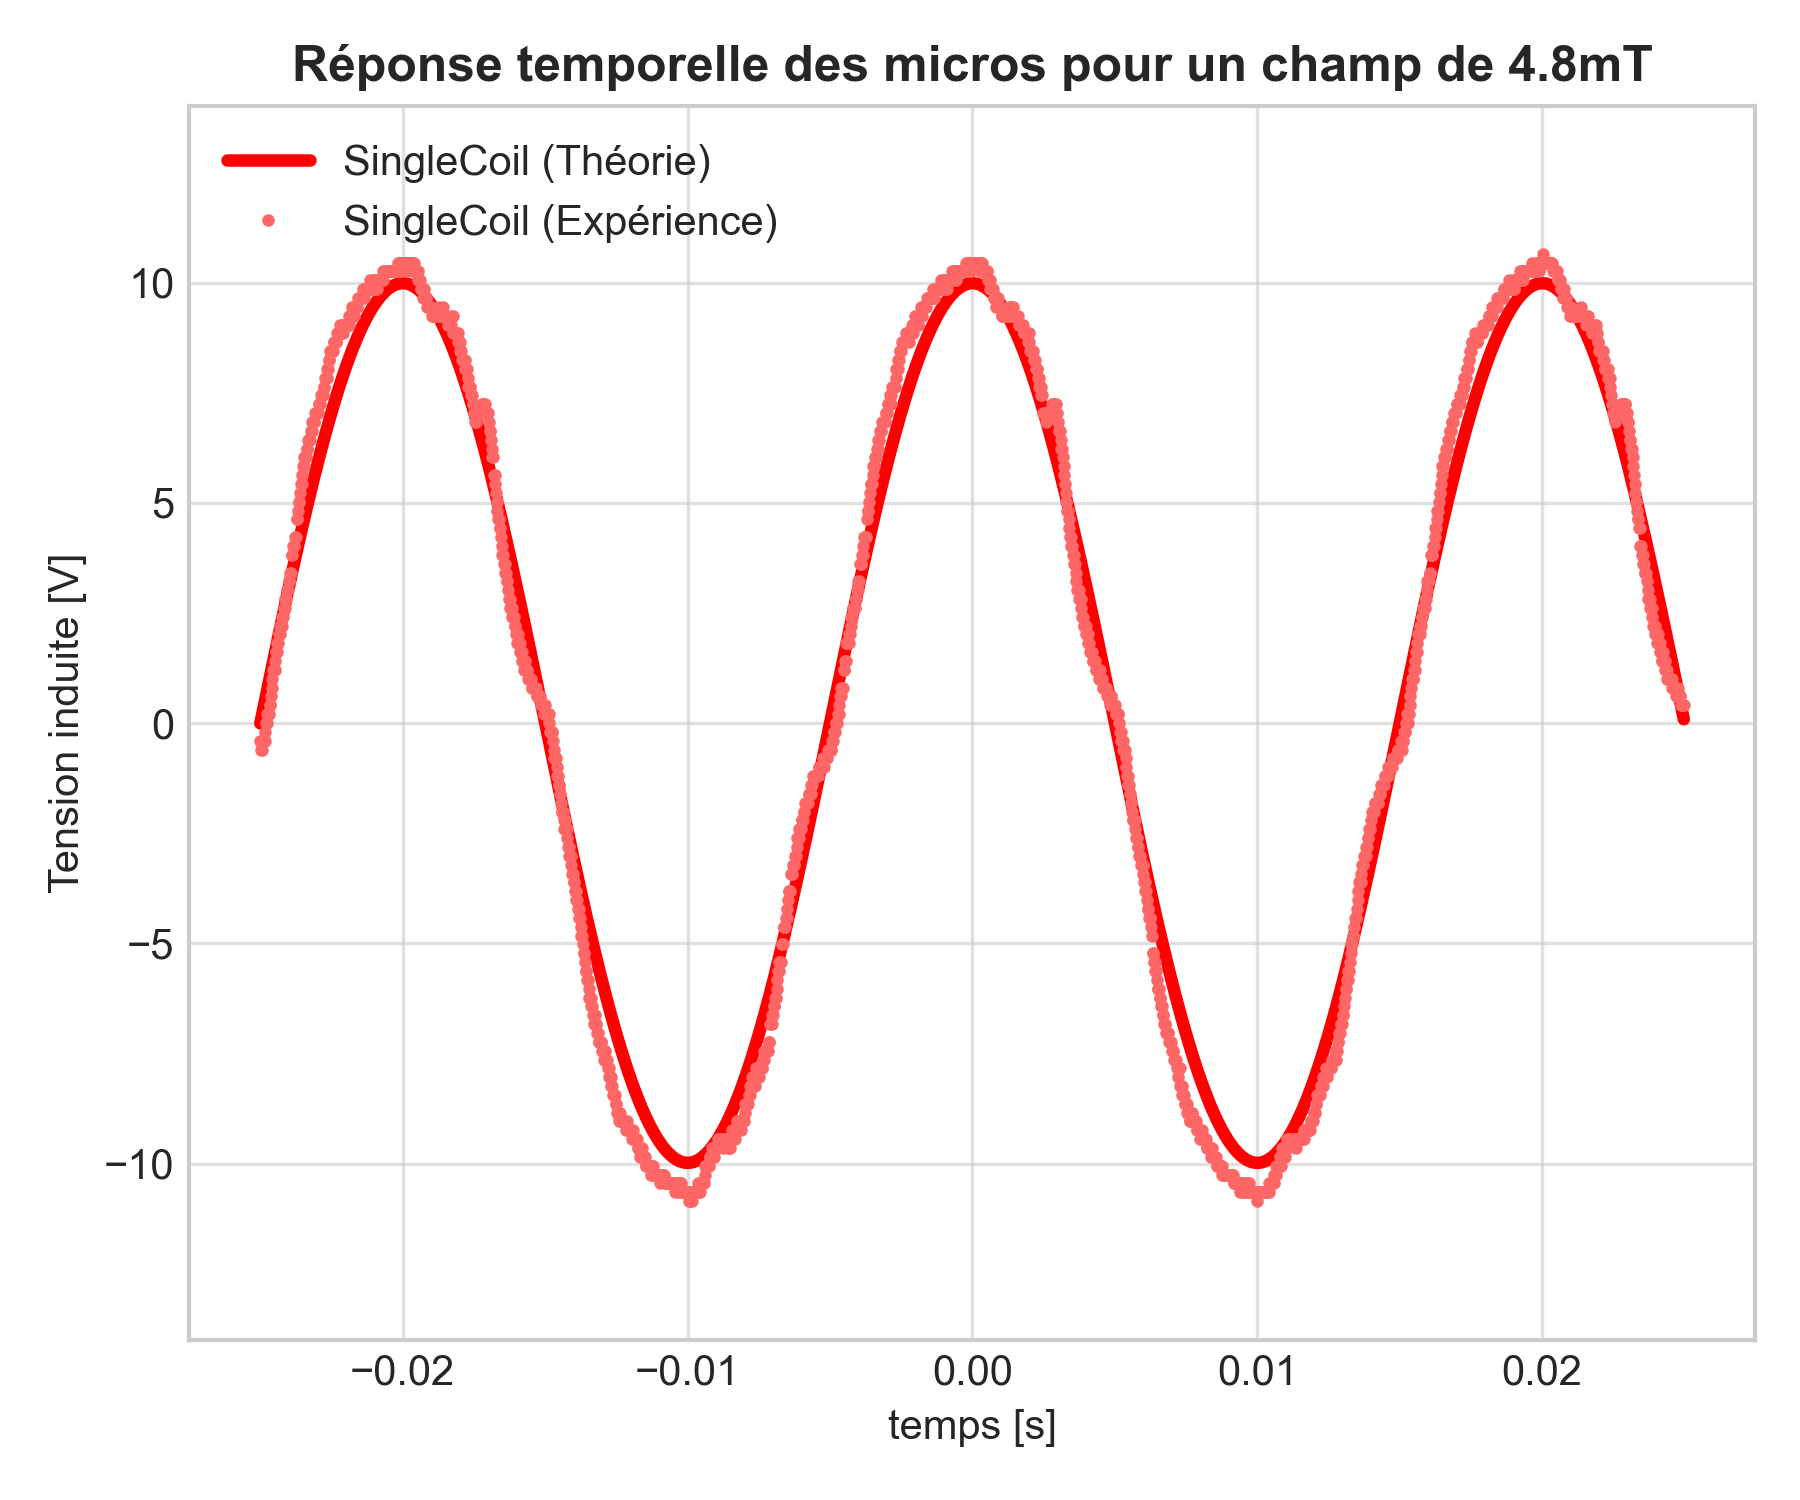
\includegraphics[width=\linewidth]{../../../Python/Exports/03-Reponse_magnetique/Singlecoil.png}
        \caption{Time response of the pickup to an external magnetic field}
    \end{minipage}\hfill
    \begin{minipage}{0.48\textwidth}
        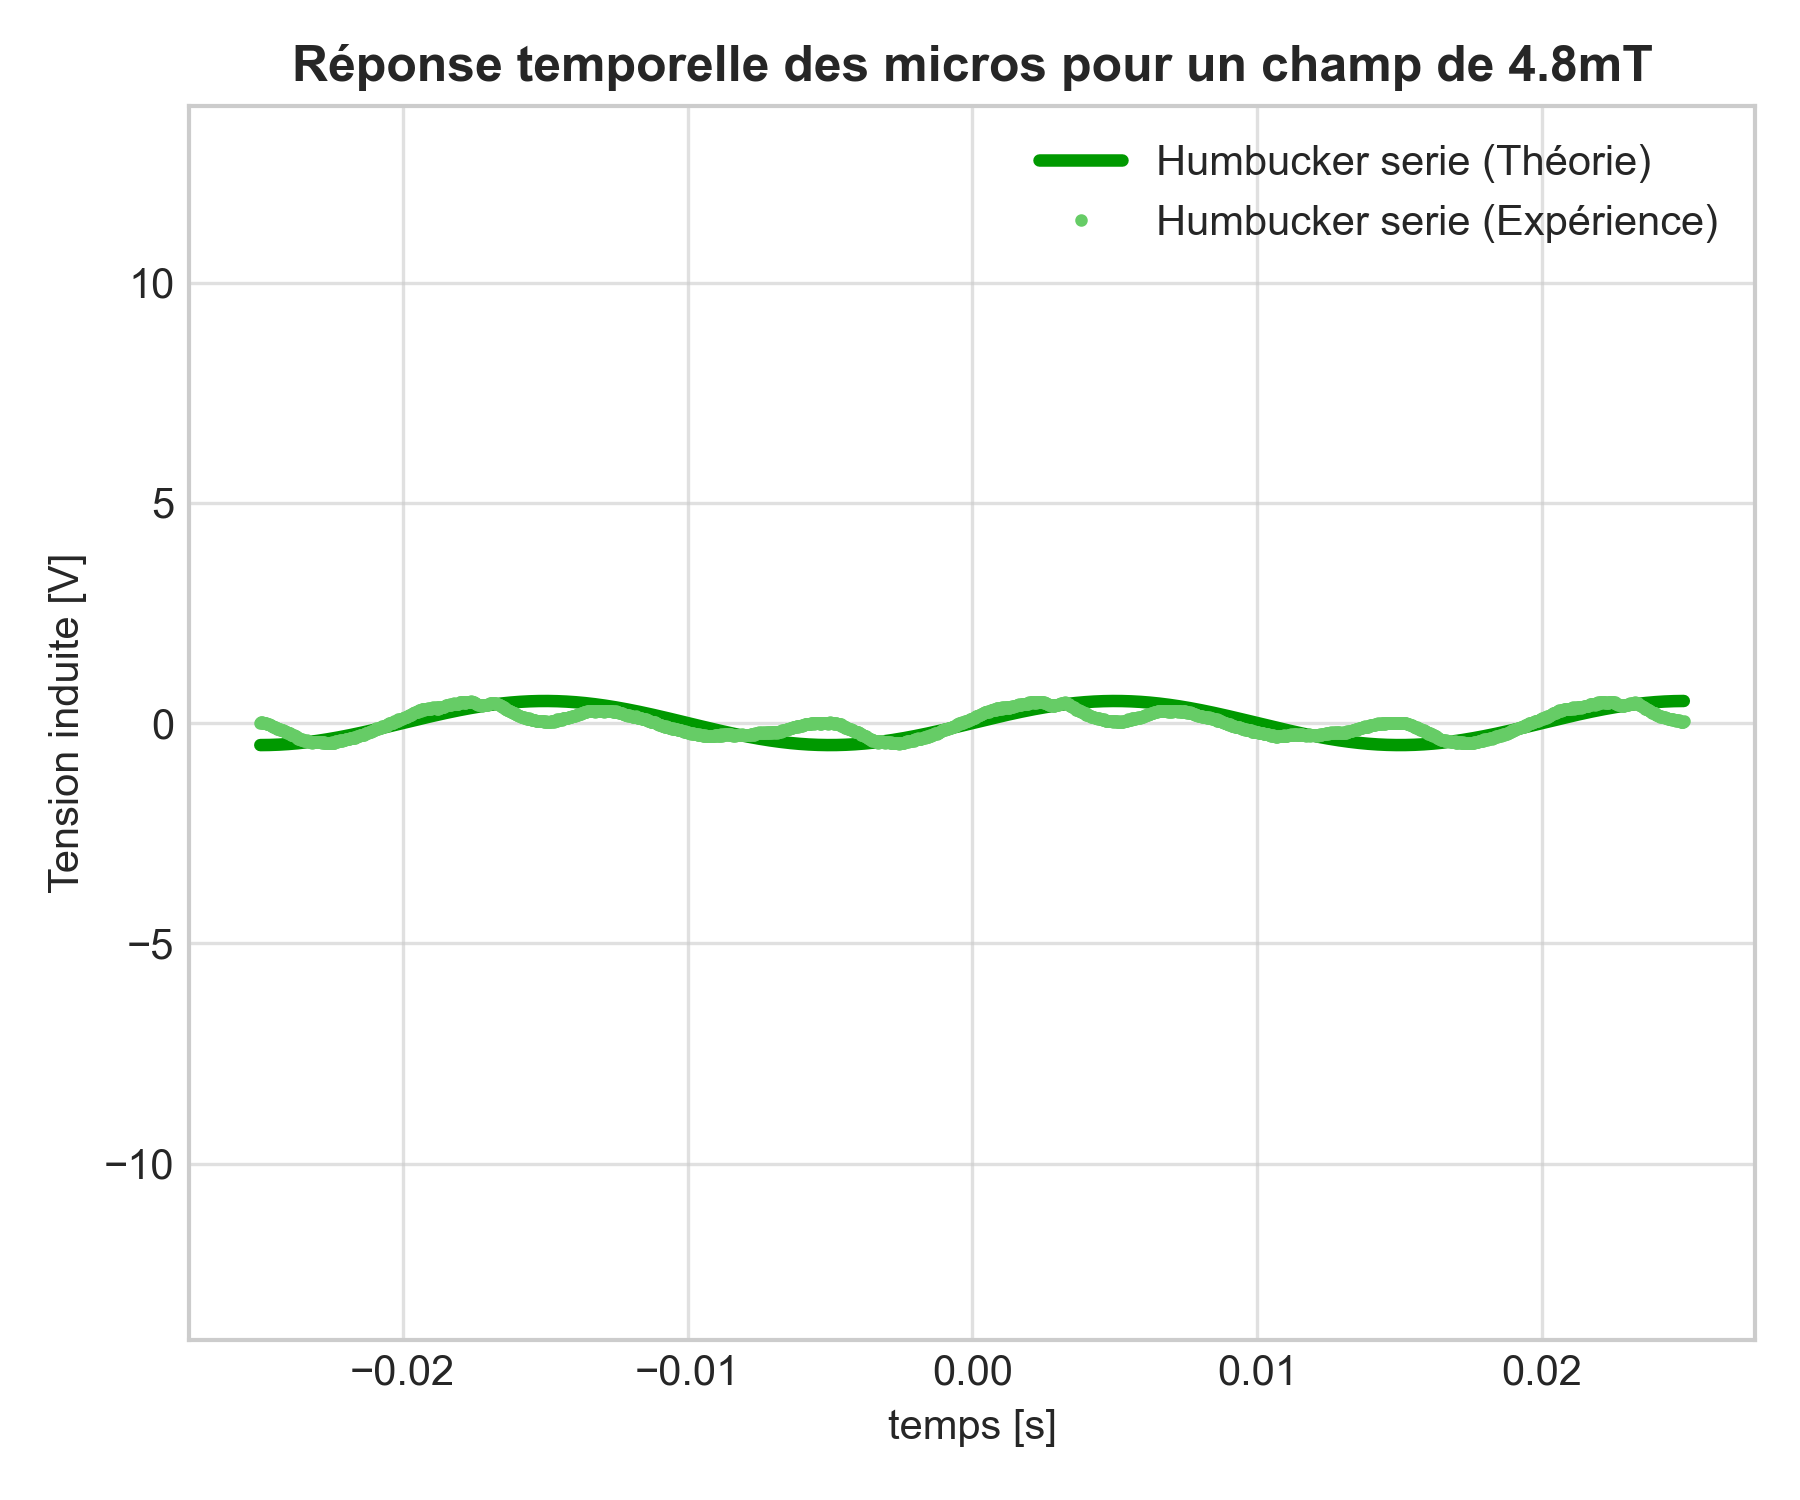
\includegraphics[width=\linewidth]{../../../Python/Exports/03-Reponse_magnetique/Humbucker.png}
        \caption{Time response of the pickup to an external magnetic field}
    \end{minipage}
\end{figure}

\subsubsection{Common-mode rejection ratio (CMRR)}
Experimental measurements reveal a sensitivity to interfering magnetic fields of $k_{Sexp} = 2,05 \text{ V}\cdot\text{mT}^{-1}$ for the SingleCoil, compared with $k_{Hpexp} = 1,37 \text{ V}\cdot\text{mT}^{-1}$ for the parallel Humbucker and $k_{Hsexp} = 0,08 \text{ V}\cdot\text{mT}^{-1}$ (Fig. 12). Although this attenuation confirms the Humbucker's relative effectiveness, the absolute value of $k_{Hpexp}$ remains high, corroborating the idea that the tested pickup has an asymmetric winding.

This reduction in sensitivity is quantified by the common-mode rejection ratio (CMRR). The significant difference between the theoretical CMRR (39.3 dB) and the experimental value (3.5 dB) highlights the practical limitations of perfect interference cancellation. Several factors explain this divergence, including winding-construction asymmetries detected in Part I and imperfections in the experimental setup, which introduce asymmetries in exposure to the interfering field.

Despite these limitations, the results validate the Humbucker's superiority in preserving signal purity in a noisy environment, particularly in the presence of low-frequency magnetic interference (e.g., 50 Hz). This study thus emphasizes the importance of mechanical and electrical design in optimizing noise-rejection performance, while confirming that ideal theoretical models must be adapted to real manufacturing constraints.

\begin{figure}[H]
    \centering
    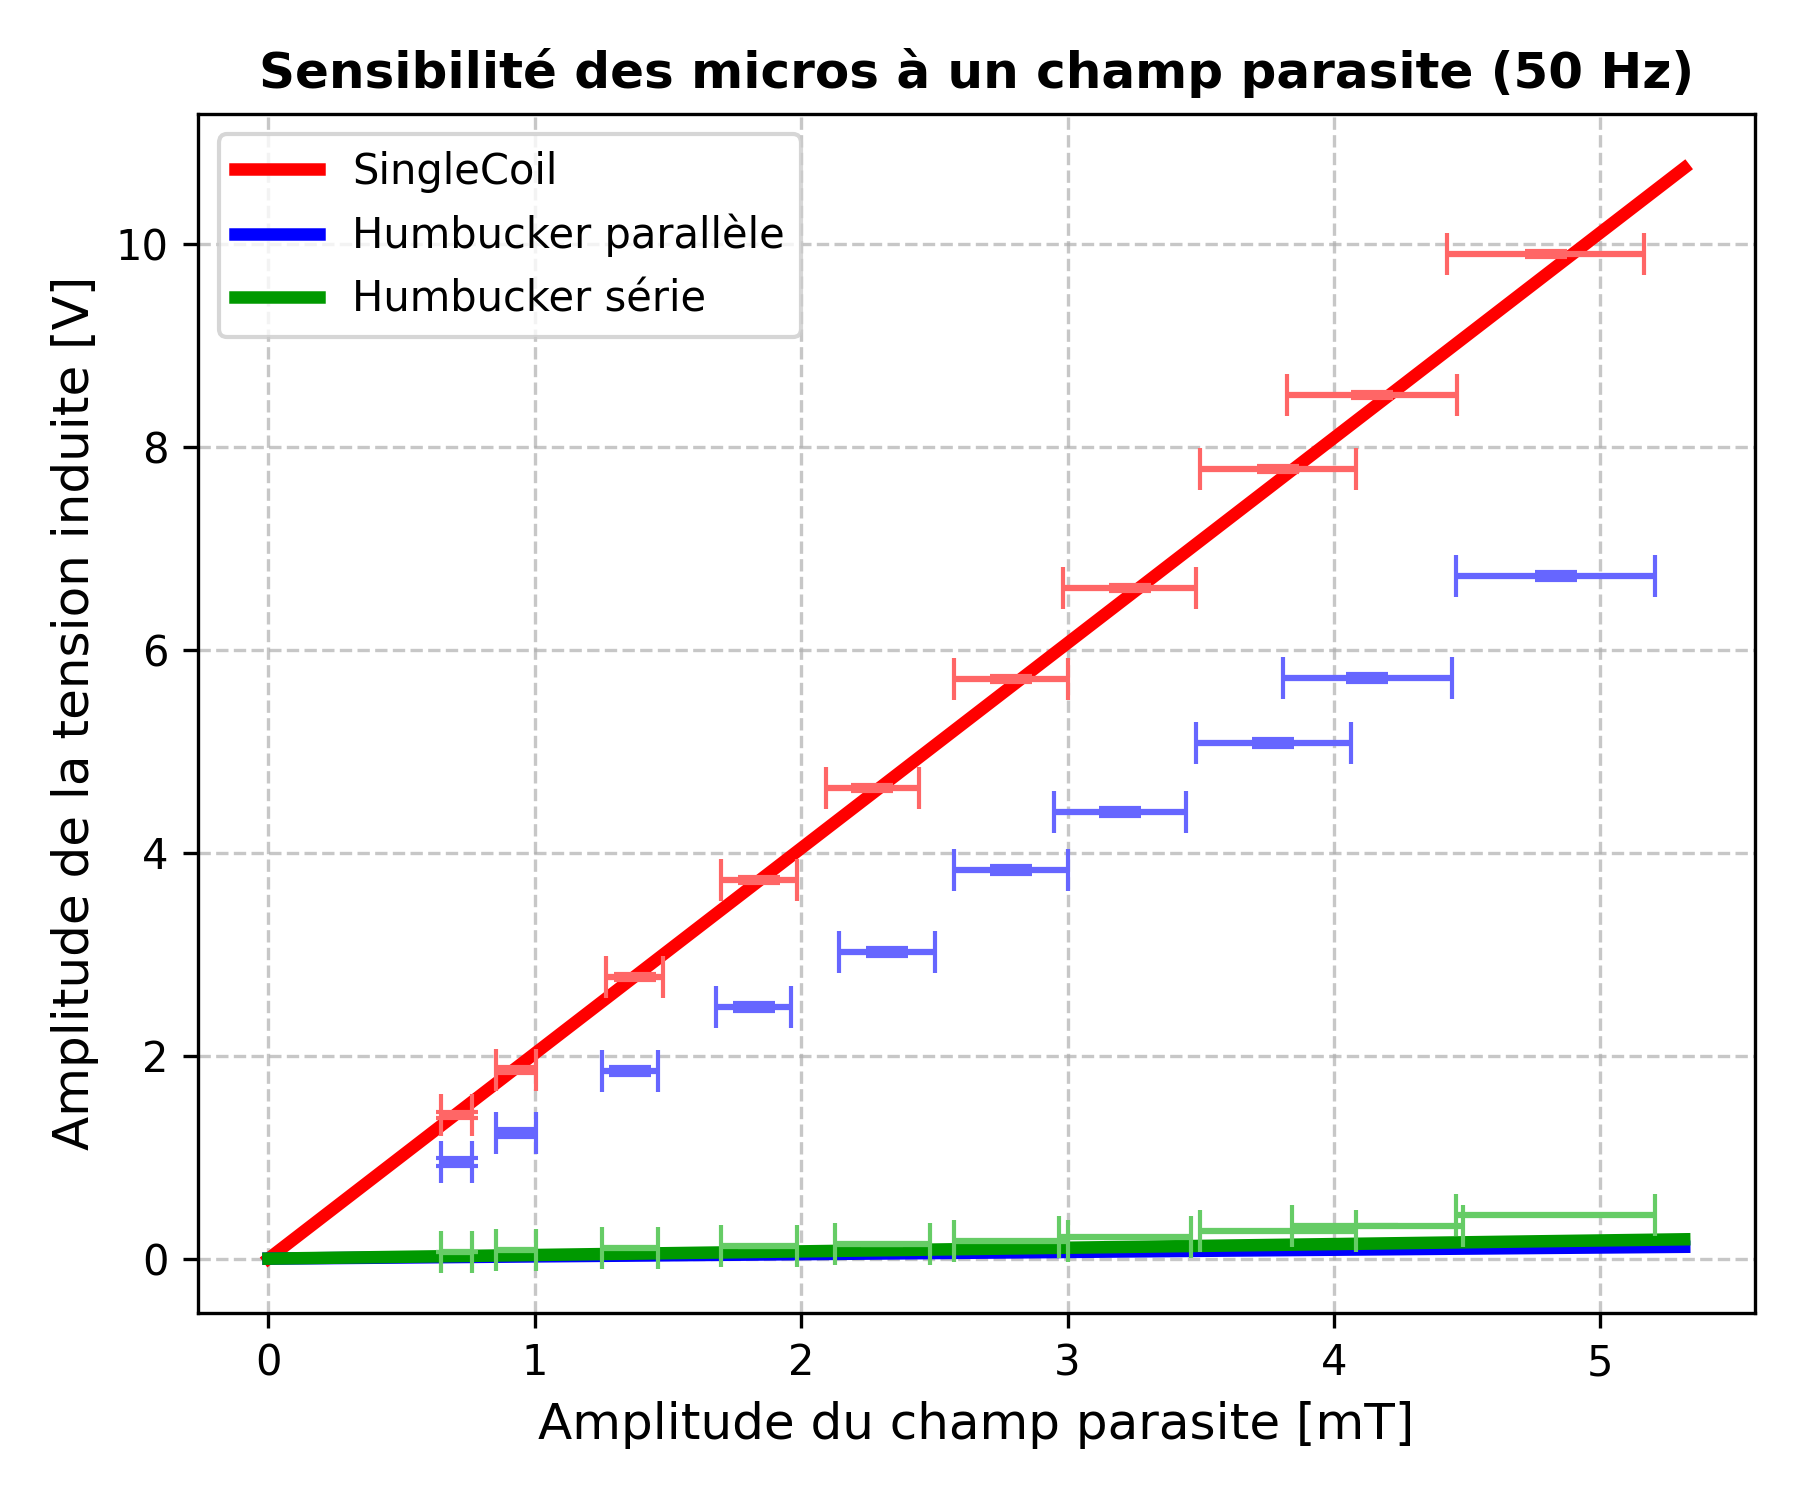
\includegraphics[width=0.8\textwidth]{../../../Python/Exports/03-Reponse_magnetique/Droite_de_sensibilite.png}
    \caption{Pickup sensitivity to an external magnetic field}
\end{figure}

\subsection{Conclusion}
The analysis of electromagnetic-interference rejection demonstrates the functional advantage of the Humbucker pickup, particularly in demanding high-amplification contexts. Acoustically, this technology significantly attenuates 50 Hz hum, a ubiquitous source of interference in stage and studio environments. Unlike the SingleCoil, whose high sensitivity to ambient magnetic fields degrades signal quality, the Humbucker ensures greater sonic clarity even in the presence of intense electromagnetic interference.

For the guitarist, this characteristic results in a cleaner sound environment, essential for using high gain levels without interference. The Humbucker is therefore not limited to a simple technical improvement: it offers greater artistic freedom by enabling robust amplification and precise control of timbre, even under unfavorable electromagnetic conditions.

This study confirms that the choice between SingleCoil and Humbucker is not merely a matter of sound preference, but also a technical compromise between harmonic richness and immunity to interference, a central issue for musicians and instrument makers.

\newpage
% --- SECTION IV ---
\section{Conclusion}
This comparative study provides a quantitative and qualitative answer to the question of how winding type influences the performance of electric guitar pickups. The objective was to assess the extent to which adding a second coil to the Humbucker makes it possible to combine the elimination of electromagnetic interference with preservation of the induced signal's spectral richness.

The results demonstrate that the pickup behaves as a second-order low-pass filter whose frequency response depends on its intrinsic parameters. Identification using the least-squares algorithm reveals that the SingleCoil has a pronounced resonance peak, favoring high frequencies and giving the sound its characteristic brightness. The parallel Humbucker offers a more linear response, but without harmonic reinforcement in the audible spectrum, explaining its ``darker'' timbre. The series Humbucker represents a compromise between the two, with attenuated resonance but better preservation of the midrange.

Analysis of induction and spatial filtering highlights the influence of the Humbucker's dual geometry. The spacing $\Delta$ between the coils produces comb filtering, selectively attenuating certain harmonics of the vibrating string. Unlike the SingleCoil, which faithfully captures the mechanical vibration, the Humbucker actively modifies the signal's spectral content. This phenomenon confirms that the observed loss of brightness is not solely electrical in origin, but also results from destructive interference inherent in its spatial design.

Evaluation of the common-mode rejection ratio (CMRR) validates the Humbucker's effectiveness in reducing interference. Although the experimental measurements reveal a CMRR of 3.5 dB (compared with 393 dB in theory), the attenuation of 50 Hz hum remains significant for the series Humbucker.

For the guitarist, choosing between SingleCoil and Humbucker represents a fundamental compromise. The SingleCoil offers harmonic richness and brightness suited to styles requiring great expressiveness (e.g., blues, funk). The Humbucker, meanwhile, guarantees sonic stability and immunity to interference, which are essential in high-gain environments (e.g., metal, jazz with heavy amplification).

\newpage
\section{Notation and numerical values}
\subsection{Electrical and mechanical characteristics}
\begin{center}
\small
\begin{tabularx}{\textwidth}{llcX}
\toprule
\textbf{Notation} & \textbf{Value} & \textbf{Unit} & \textbf{Description} \\
\midrule
$\mu_{0}$ & $4\pi \cdot 10^{-7}$ & H$\cdot$m$^{-1}$ & Magnetic permeability of vacuum \\
$\mu_{r}$ & 2 & -- & Relative permeability of Alnico 5 \\
\midrule
$R_{s_S}$ & $5,26 \cdot 10^3$ & $\Omega$ & Internal resistance of the SingleCoil pickup \\
$L_{S}$ & 2,37 & H & Inductance of the SingleCoil pickup \\
$C_{S}$ & $0,37 \cdot 10^{-9}$ & F & Internal capacitance of the SingleCoil pickup \\
$R_{p_S}$ & $492,3 \cdot 10^3$ & $\Omega$ & Eddy-current loss resistance \\
\midrule
$R_{s_{\text{Hp}}}$ & $4,52 \cdot 10^3$ & $\Omega$ & Internal resistance of the parallel Humbucker pickup \\
$L_{\text{Hp}}$ & 1,72 & H & Inductance of the parallel Humbucker pickup \\
$C_{\text{Hp}}$ & $0,05 \cdot 10^{-9}$ & F & Internal capacitance of the parallel Humbucker pickup \\
$R_{p_{\text{Hp}}}$ & $343,0 \cdot 10^3$ & $\Omega$ & Eddy-current loss resistance \\
\midrule
$R_{s_{\text{Hs}}}$ & $15,10 \cdot 10^3$ & $\Omega$ & Internal resistance of the series Humbucker pickup \\
$L_{\text{Hs}}$ & $4,60$ & H & Inductance of the series Humbucker pickup \\
$C_{\text{Hs}}$ & $0,11 \cdot 10^{-9}$ & F & Internal capacitance of the series Humbucker pickup \\
$R_{p_{\text{Hs}}}$ & $1,05 \cdot 10^6$ & $\Omega$ & Eddy-current loss resistance \\
\midrule
$x_{S}$ & 0,105 & m & Position of the SingleCoil pickup \\
$x_{\text{Hp1}}, x_{\text{Hp2}}$ & 0,147 - 0,165 & m & Position of the coils of the parallel Humbucker \\
$x_{\text{Hs1}}, x_{\text{Hs2}}$ & 0,202 - 0,220 & m & Position of the coils of the series Humbucker \\
$\Delta$ & 0,018 & m & Center-to-center distance between the two Humbucker coils \\
\midrule
$z_{0}$ & 0,004 & m & String-to-pickup distance at rest \\
$L$ & 0,85 & m & Length of the vibrating string \\
$x_{0}$ & 0,20 & m & Position of the perturbation origin \\
$A_{0}$ & 0,005 (ODG) & m & Initial amplitude of the perturbation \\
$F$ & 80 & Hz & Fundamental frequency of string vibration \\
\bottomrule
\end{tabularx}
\end{center}

\subsection{Magnetic characteristics}
\begin{center}
\small
\begin{tabularx}{\textwidth}{llcX}
\toprule
\textbf{Notation} & \textbf{Value} & \textbf{Unit} & \textbf{Description} \\
\midrule
$\chi$ & 100 (ODG) & -- & Magnetic susceptibility of the string \\
$V$ & $1 \cdot 10^{-8}$ (ODG) & m$^{3}$ & Volume of the active portion of the string \\
\midrule
$F_{B}$ & 50 & Hz & Frequency of the interfering magnetic field \\
$\alpha$ & 1 (ODG) & m$^{-1}$ & Gradient of the interfering magnetic field \\
\midrule
$k_{s}$ & 2,02 & $V.mT^{-1}$ & Theoretical sensitivity of the SingleCoil \\
$k_{\text{Hp}}$ & 0,02 & $V.mT^{-1}$ & Theoretical sensitivity of the parallel Humbucker \\
$k_{\text{Hs}}$ & 0,04 & $V.mT^{-1}$ & Theoretical sensitivity of the series Humbucker \\
$k_{\text{Sexp}}$ & 2,05 & $V.mT^{-1}$ & Experimental sensitivity of the SingleCoil \\
$k_{\text{Hpexp}}$ & 1,37 & $V.mT^{-1}$ & Experimental sensitivity of the parallel Humbucker \\
$k_{\text{Hsexp}}$ & 0,08 & $V.mT^{-1}$ & Experimental sensitivity of the series Humbucker \\
\midrule
$\text{CMRR}_{Hp}$ & 39,3 & dB & Theoretical CMRR of the parallel Humbucker \\
$\text{CMRR}_{Hs}$ & 35,0 & dB & Theoretical CMRR of the series Humbucker \\
$\text{CMRR}_{\text{Hpexp}}$ & 3,5 & dB & Experimental CMRR of the parallel Humbucker \\
$\text{CMRR}_{\text{Hsexp}}$ & 28,7 & dB & Experimental CMRR of the series Humbucker \\
\bottomrule
\end{tabularx}
\end{center}

\newpage
% --- REFERENCES ---
\begin{thebibliography}{9}

\bibitem{wiseguy} 
WiseGuy Research Consultants, \textit{"Global Electric Guitar Pickup Market Research Report 2024,"} Pune, India, 2024.

\bibitem{hill} 
Matthew W. Hill, \textit{"The hidden history of the electric guitar"}, in \textit{Quand la guitare [s']électrise!}, Benoît Navarret et al. (dir.), Sorbonne Université Presses, pp. 33-61, 2022.

\bibitem{horton} 
N. G. Horton \& T. R. Moore: \textit{Modeling the magnetic pickup of an electric guitar} : American Journal of Physics, vol. 77, no. 2, pp. 144-150, 2009, doi: 10.1119/1.2990663.

\bibitem{duncan} 
S. W. Duncan, \textit{"Interview With Seth Lover"}, Seymour Duncan. [En ligne]. Disponible sur : \url{www.seymourduncan.com/blog/latest-updates/seymour-w-duncans-interview-with-seth-lover}

\bibitem{carson} 
Dan Carson, \textit{"Investigation of the Electromagnetic Properties of Electric Guitar Pickups"}, University of Illinois at Urbana-Champaign, Physics Senior Thesis, 2009.

\bibitem{andrea} 
B. d'Andréa-Novel, B. Fabre, et P. Jouvelot, \textit{Acoustique Informatique MusiquE : Outils scientifiques pour la musique}. Paris, France : Presses des Mines, 2010, ch. 4.

\end{thebibliography}

\end{document}
